\documentclass[aspectratio=169]{beamer}
    
    %%%% Heading
    
    %%% Packages 
    \usepackage{etoolbox}
    \usepackage{environ}
    \usepackage{xcolor}



    %%%%-----------------------------------_
    %%%%%% ---- Settting for all frames
    %%%%-----------------------------------_
    \BeforeBeginEnvironment{frame}{%
        \normalsize%
        \normalcolor%
    }
    
        %%%%% ----- Get rid of the Bottons
        %gets rid of bottom navigation bars
        \setbeamertemplate{footline}[frame number]{}
        
        %gets rid of bottom navigation symbols
        \setbeamertemplate{navigation symbols}{}
        
        %gets rid of footer
        %will override 'frame number' instruction above
        %comment out to revert to previous/default definitions
        \setbeamertemplate{footline}{}
    
    %%%% Margins
    \setbeamersize{text margin left=0mm,text margin right=0mm} 
    
    %%%% Points
    \definecolor{mypink1}{rgb}{0.858, 0.188, 0.478}
    \setbeamercolor{itemize item}{fg=mypink1} % all frames will have red bullets

    %%%%-----------------------------------_
    %%%%%% ---- Layouts Slides
    %%%%-----------------------------------_
    
    
    %%%%%% Set the text
    \makeatletter
        \NewEnviron{imagecolumn}{\expandafter\gdef\expandafter\imagecolcontent\expandafter{\BODY}}
        \NewEnviron{textcolumn}{\expandafter\gdef\expandafter\textcolcontent\expandafter{\BODY}}
        \newcommand{\printcolumns}{%
          \begin{columns}[T]
                \begin{column}{.3\textwidth}
                \textcolcontent
              \end{column}
              \begin{column}{.6\textwidth}
                \imagecolcontent
              \end{column}
            \end{columns}
        }
    \makeatother

    
      
    %%%% Slide
    \newenvironment{slide}[1]
    {
     \usebackgroundtemplate{\includegraphics[width=\paperwidth]{backs/#1.png}}%
     \begin{frame}[plain]
    }
    { 
    \end{frame}
    }
    
    %%%% Titulos
    \newcommand{\slidetitle}[1]{
     \begin{slide}{#1}
        \end{slide}
    }
    
    
    \graphicspath{ {./img/} }

\begin{document}
    
    %%% Titulo
    \slidetitle{1}
    
    %%% Principales Hightlihts
    \begin{frame}{Conclusiones Principales}
    
    \begin{itemize}
        \item Las brechas de ingreso por género son muy grandes, especialmente en los percentiles más bajos de ingreso.
        \item El ingreso de las mujeres está rezagado 10 años con respecto al de los hombres, en los percentiles más bajos.
        \item La tasa de mujeres jóvenes que ni estudian, ni trabajan es casi el doble que la de los hombres jóvenes. Esta brecha se agudizó con la pandemia.
    \item Gran brecha de ingreso entre minorías y no minorías  en todos los niveles de ingreso.
    \item A pesar de que la pobreza ha disminuido, las diferencias entre regiones todavía son muy altas.
    \item La pandemia del COVID-19 causó un aumento preocupante en las tasas de pobreza en las zonas urbanas, al punto de hacerla converger con la de las zonas  rurales.
    \end{itemize}

    
    \end{frame}
    
    \section{Contexto}
    %%% Contexto
    \slidetitle{2}
        

    %%% ----------------------------
    %%% Pobreza--
    %%% ----------------------------
    \subsection{Pobreza}
    
        %%%-- No monetaria
    \begin{slide}{4} 
                      \begin{imagecolumn}
                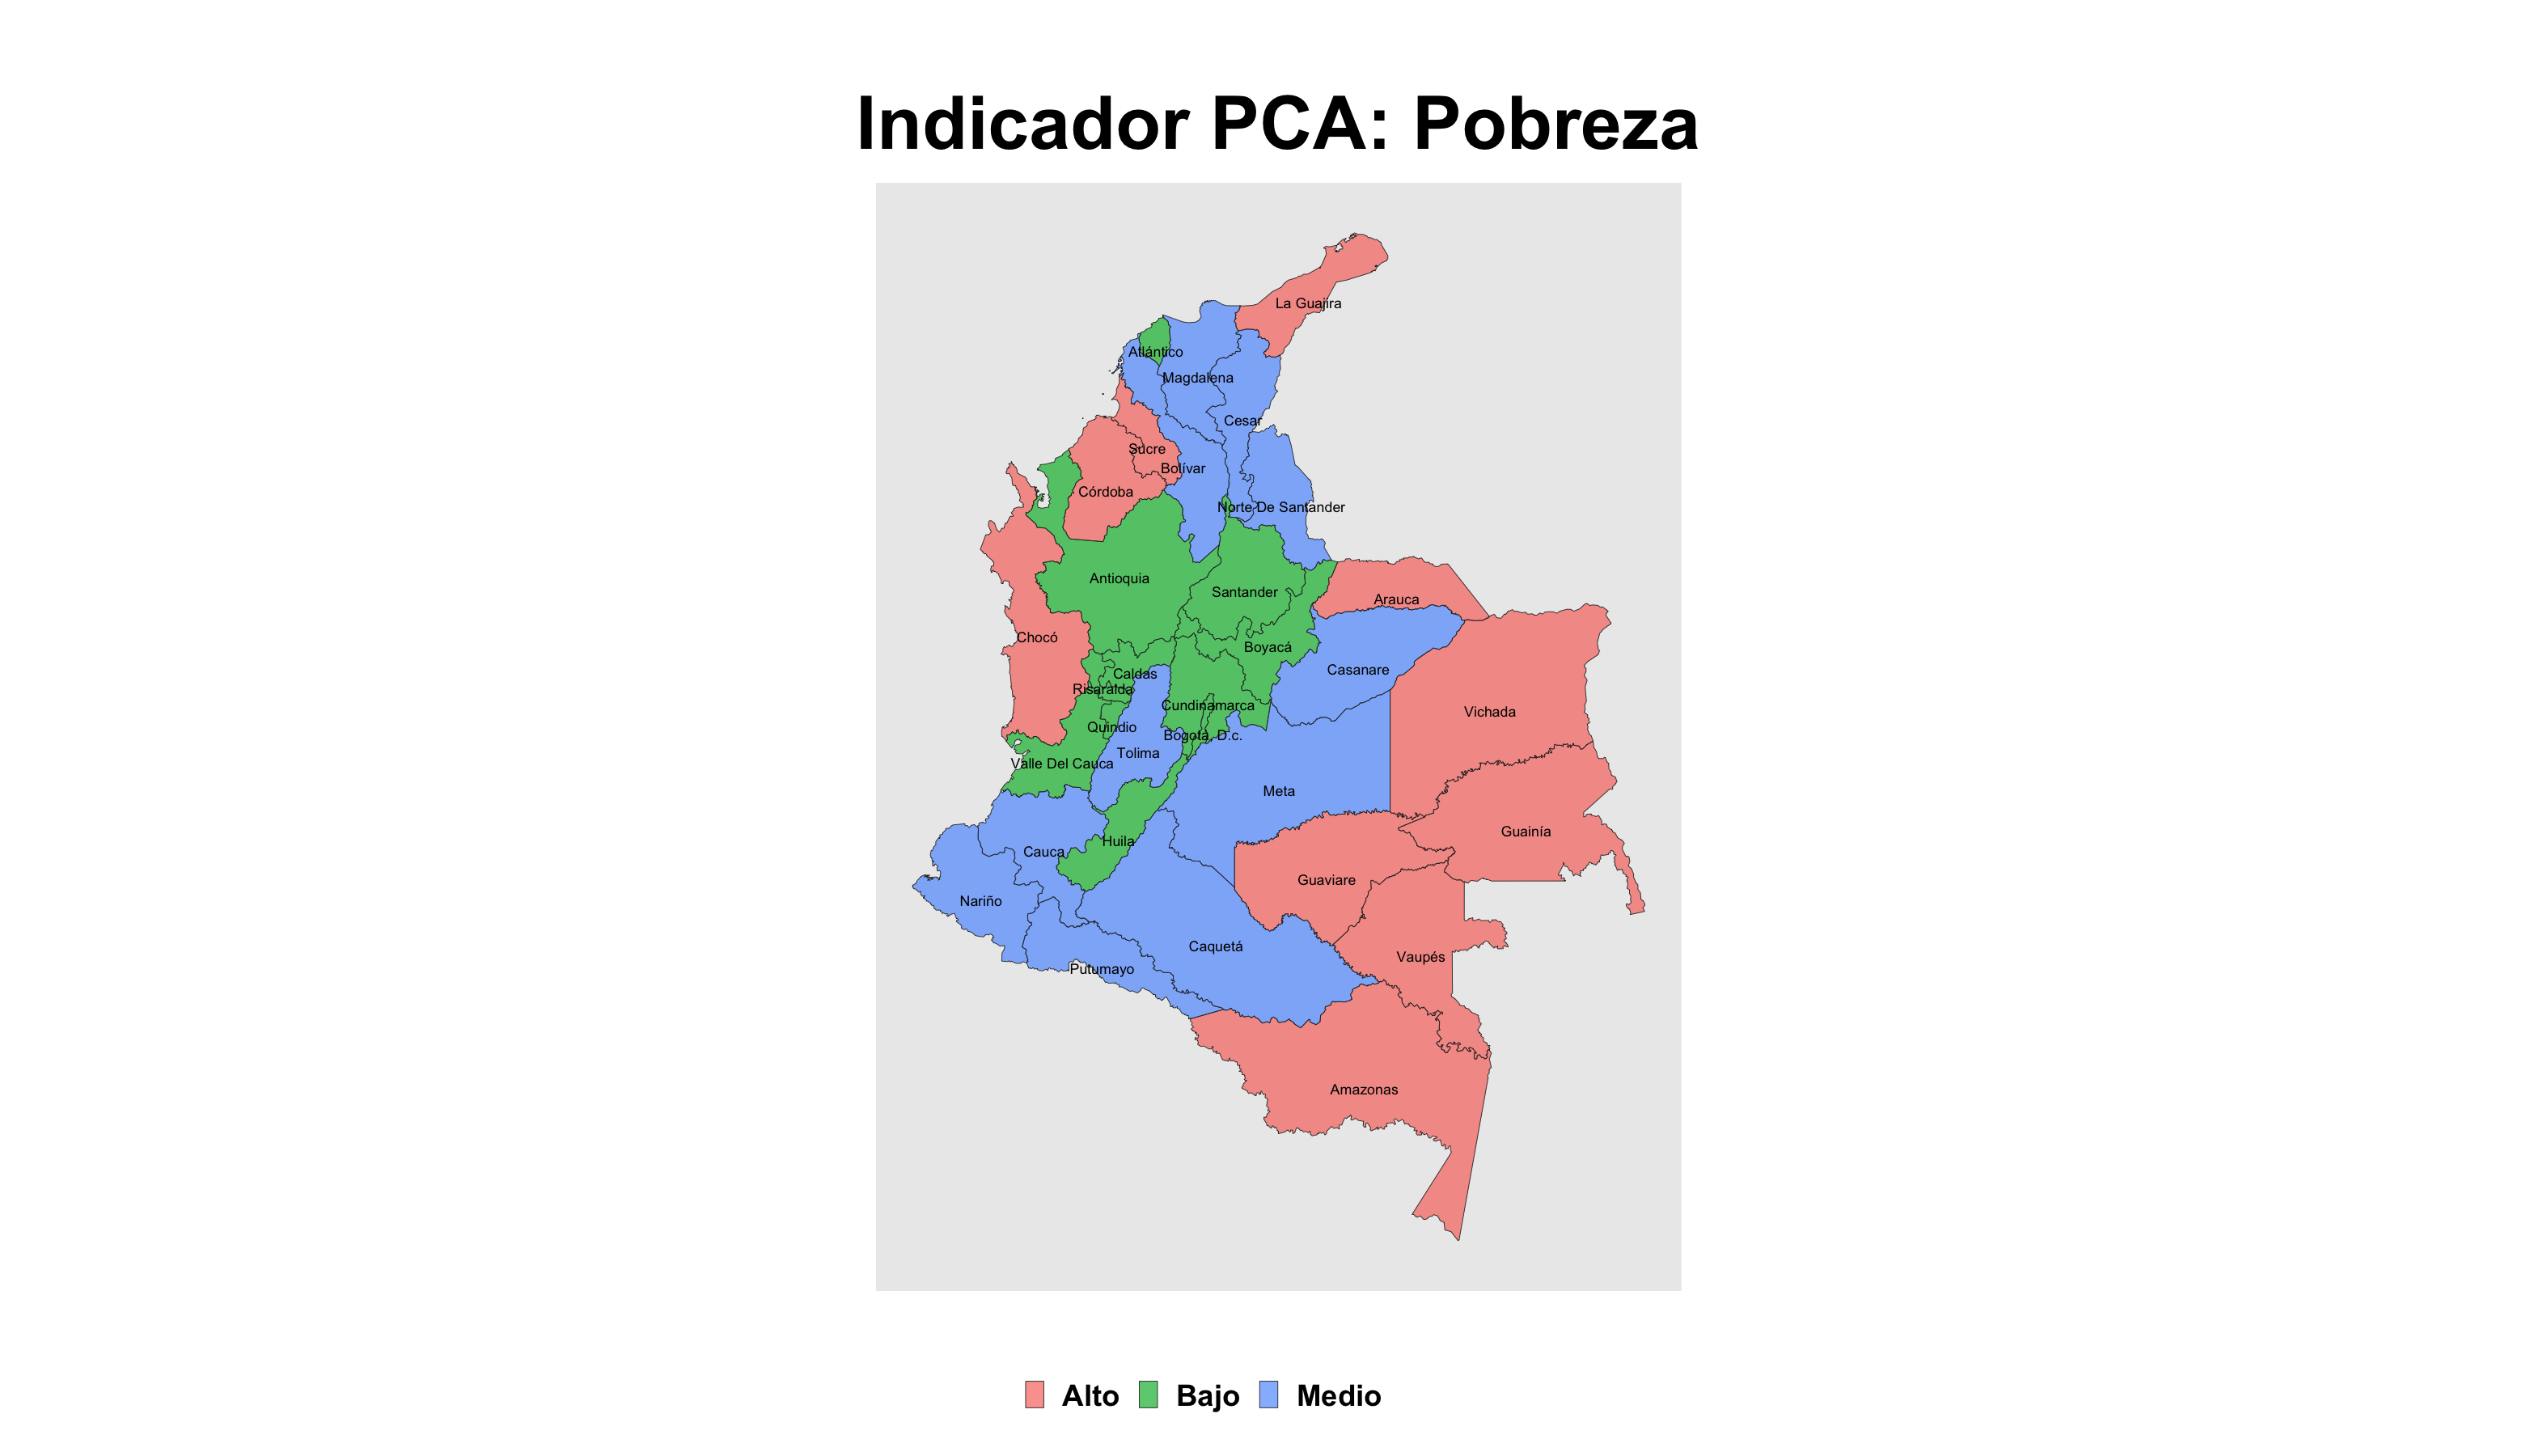
\includegraphics[width=\columnwidth]{img/pca_pobreza_pca.png}
            \end{imagecolumn}
            \begin{textcolumn}
                \begin{itemize}
                    \item A nivel nacional, existe una tendencia a la baja en la pobreza no monetaria
                    \item No obstante, las brechas territoriales son grandes y persisten.
                \end{itemize}
            \end{textcolumn}

    \printcolumns
    \end{slide}
     
  

    %%% ----------------------------
    %%% Desigualdad--
    %%% ----------------------------
    \subsection{Desigualdad}
 
     %%% Gini zonas
    \begin{slide}{5} 
            \begin{imagecolumn}
                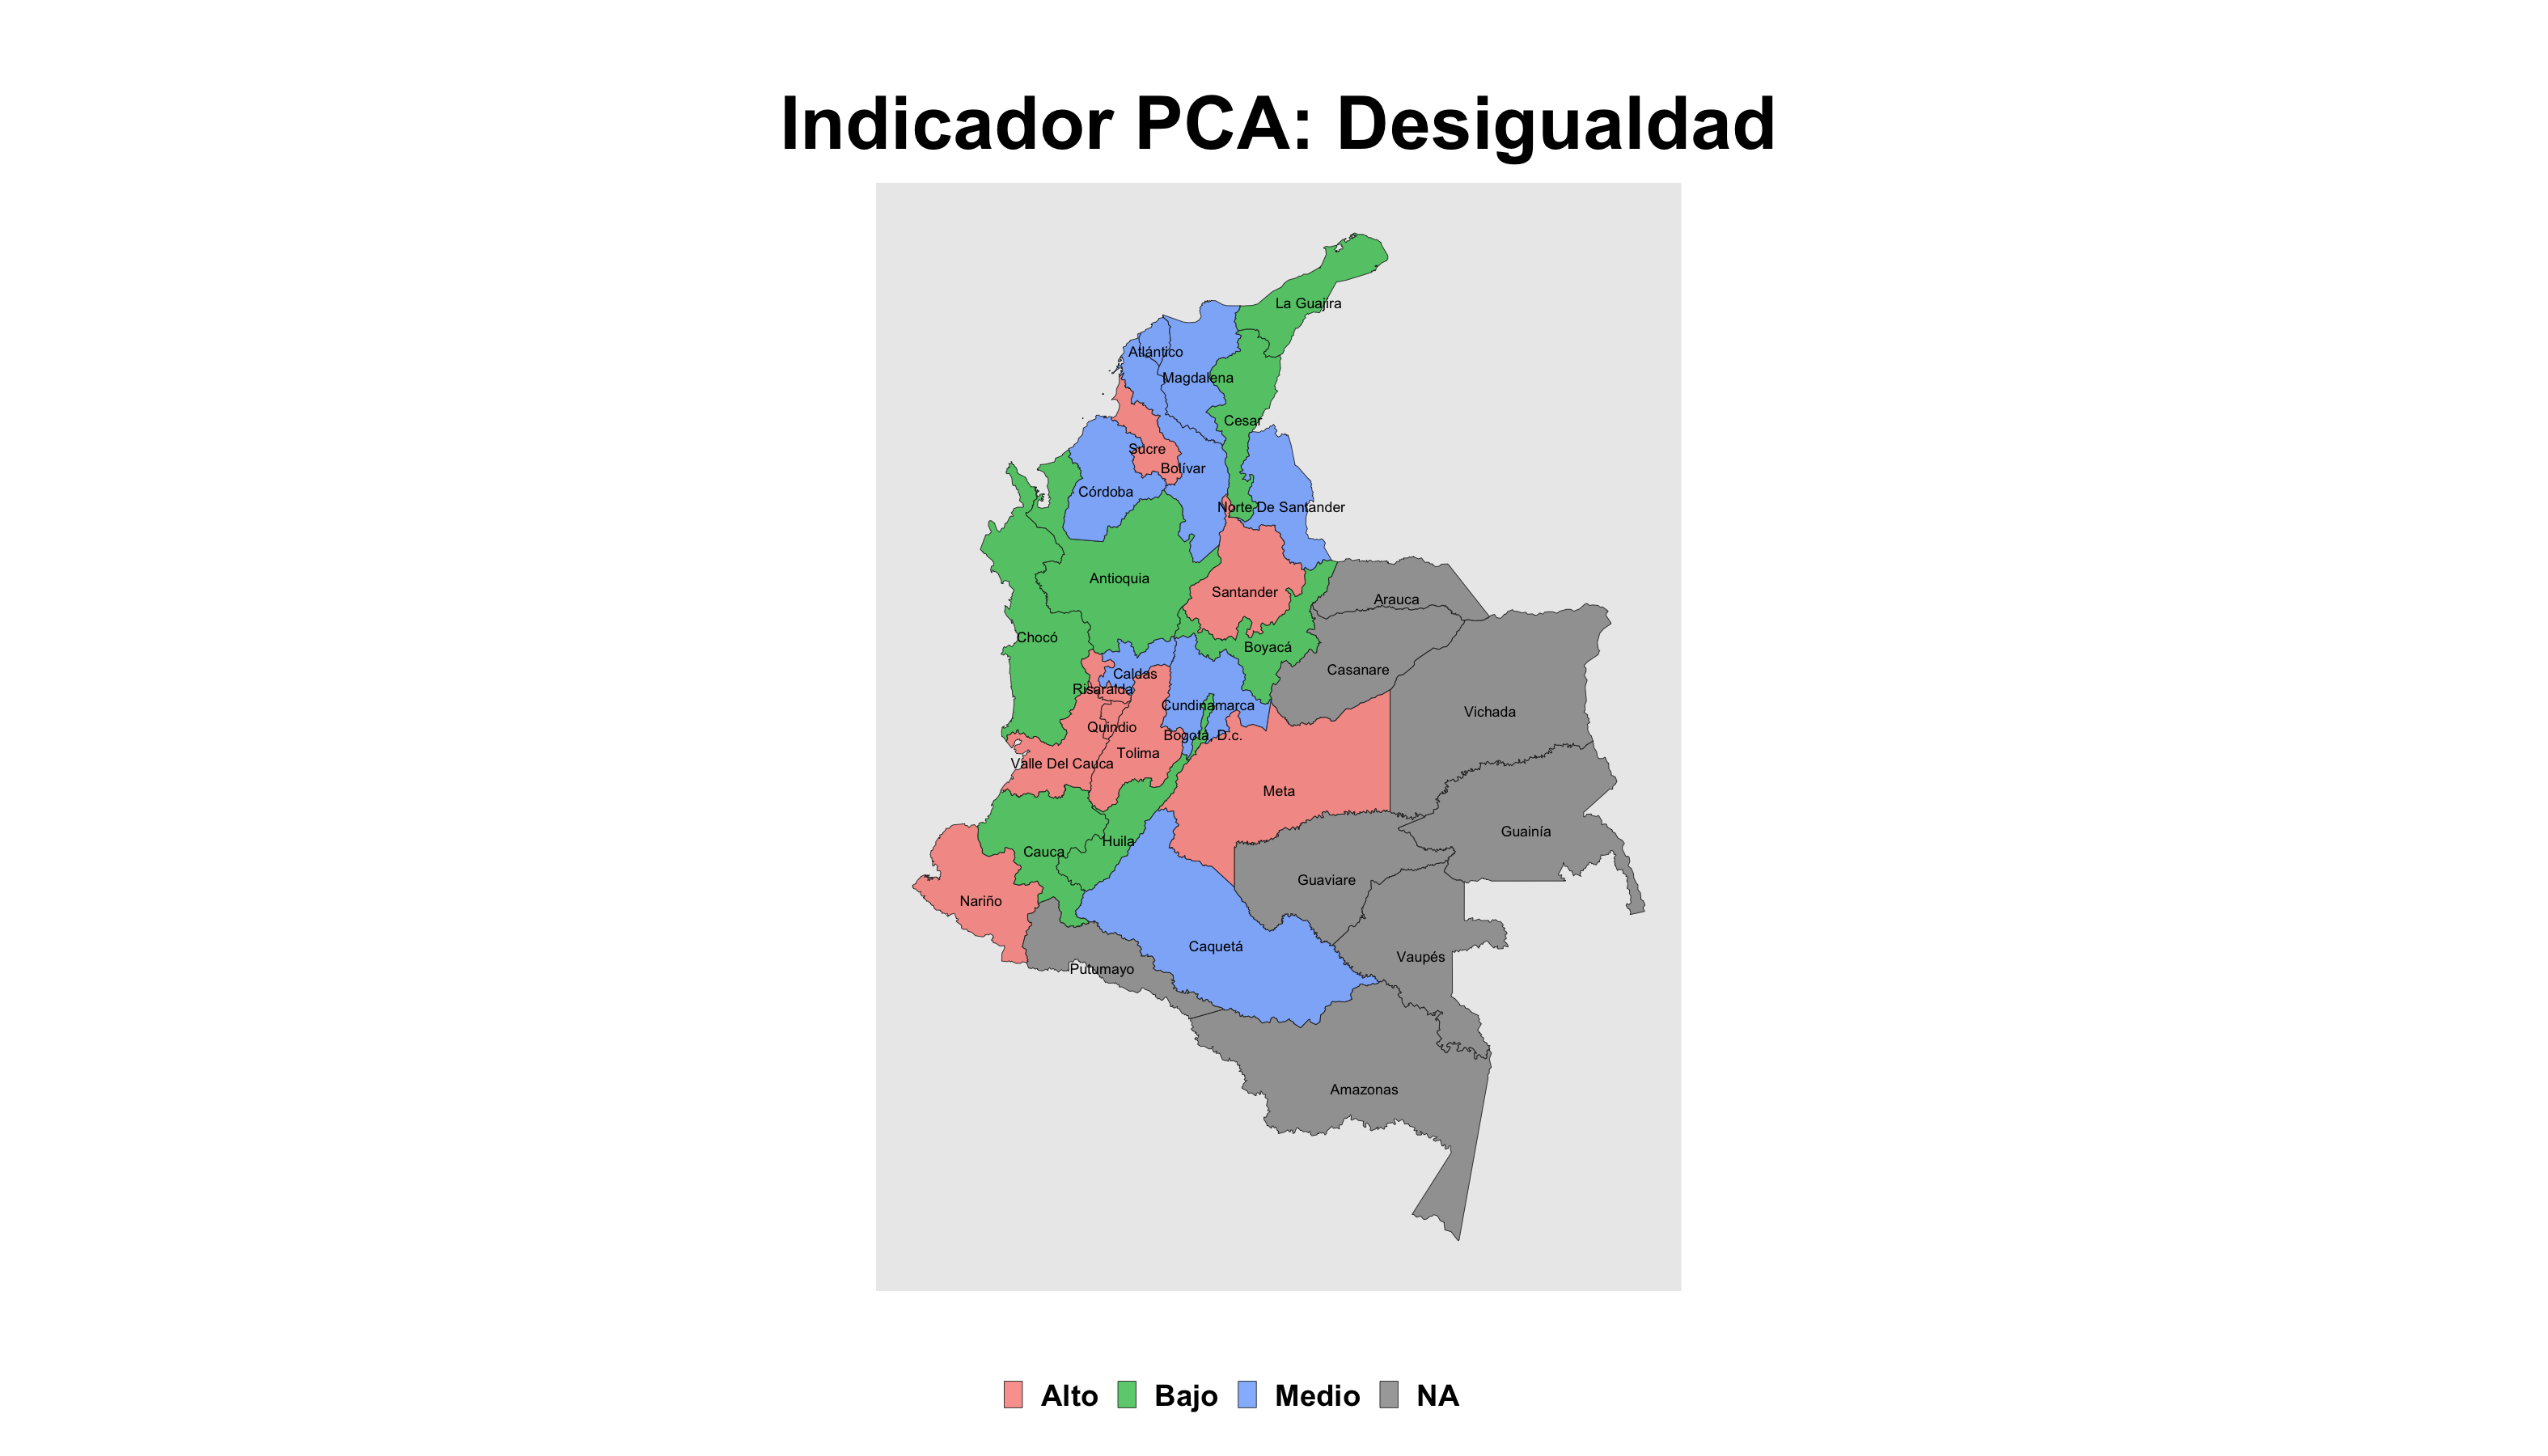
\includegraphics[width=\columnwidth]{img/pca_desigualdad_pca.png}
            \end{imagecolumn}
            \begin{textcolumn}
                \begin{itemize}
                    \item Hasta 2017 la desigualdad venia disminuyendo en todas las zonas, pero la pandemia devolvió a los territorios a los niveles de desigualdad de hace 10 años.
                \end{itemize}
            \end{textcolumn}

    \printcolumns
    \end{slide}
    
      
    
    %%% ----------------------------
    %%% Características del hogar
    %%% ----------------------------
    \subsection{Característica del hogar}
    
        %%%-- Hacinamiento Crítico 
    \begin{slide}{6} 
                      \begin{imagecolumn}
                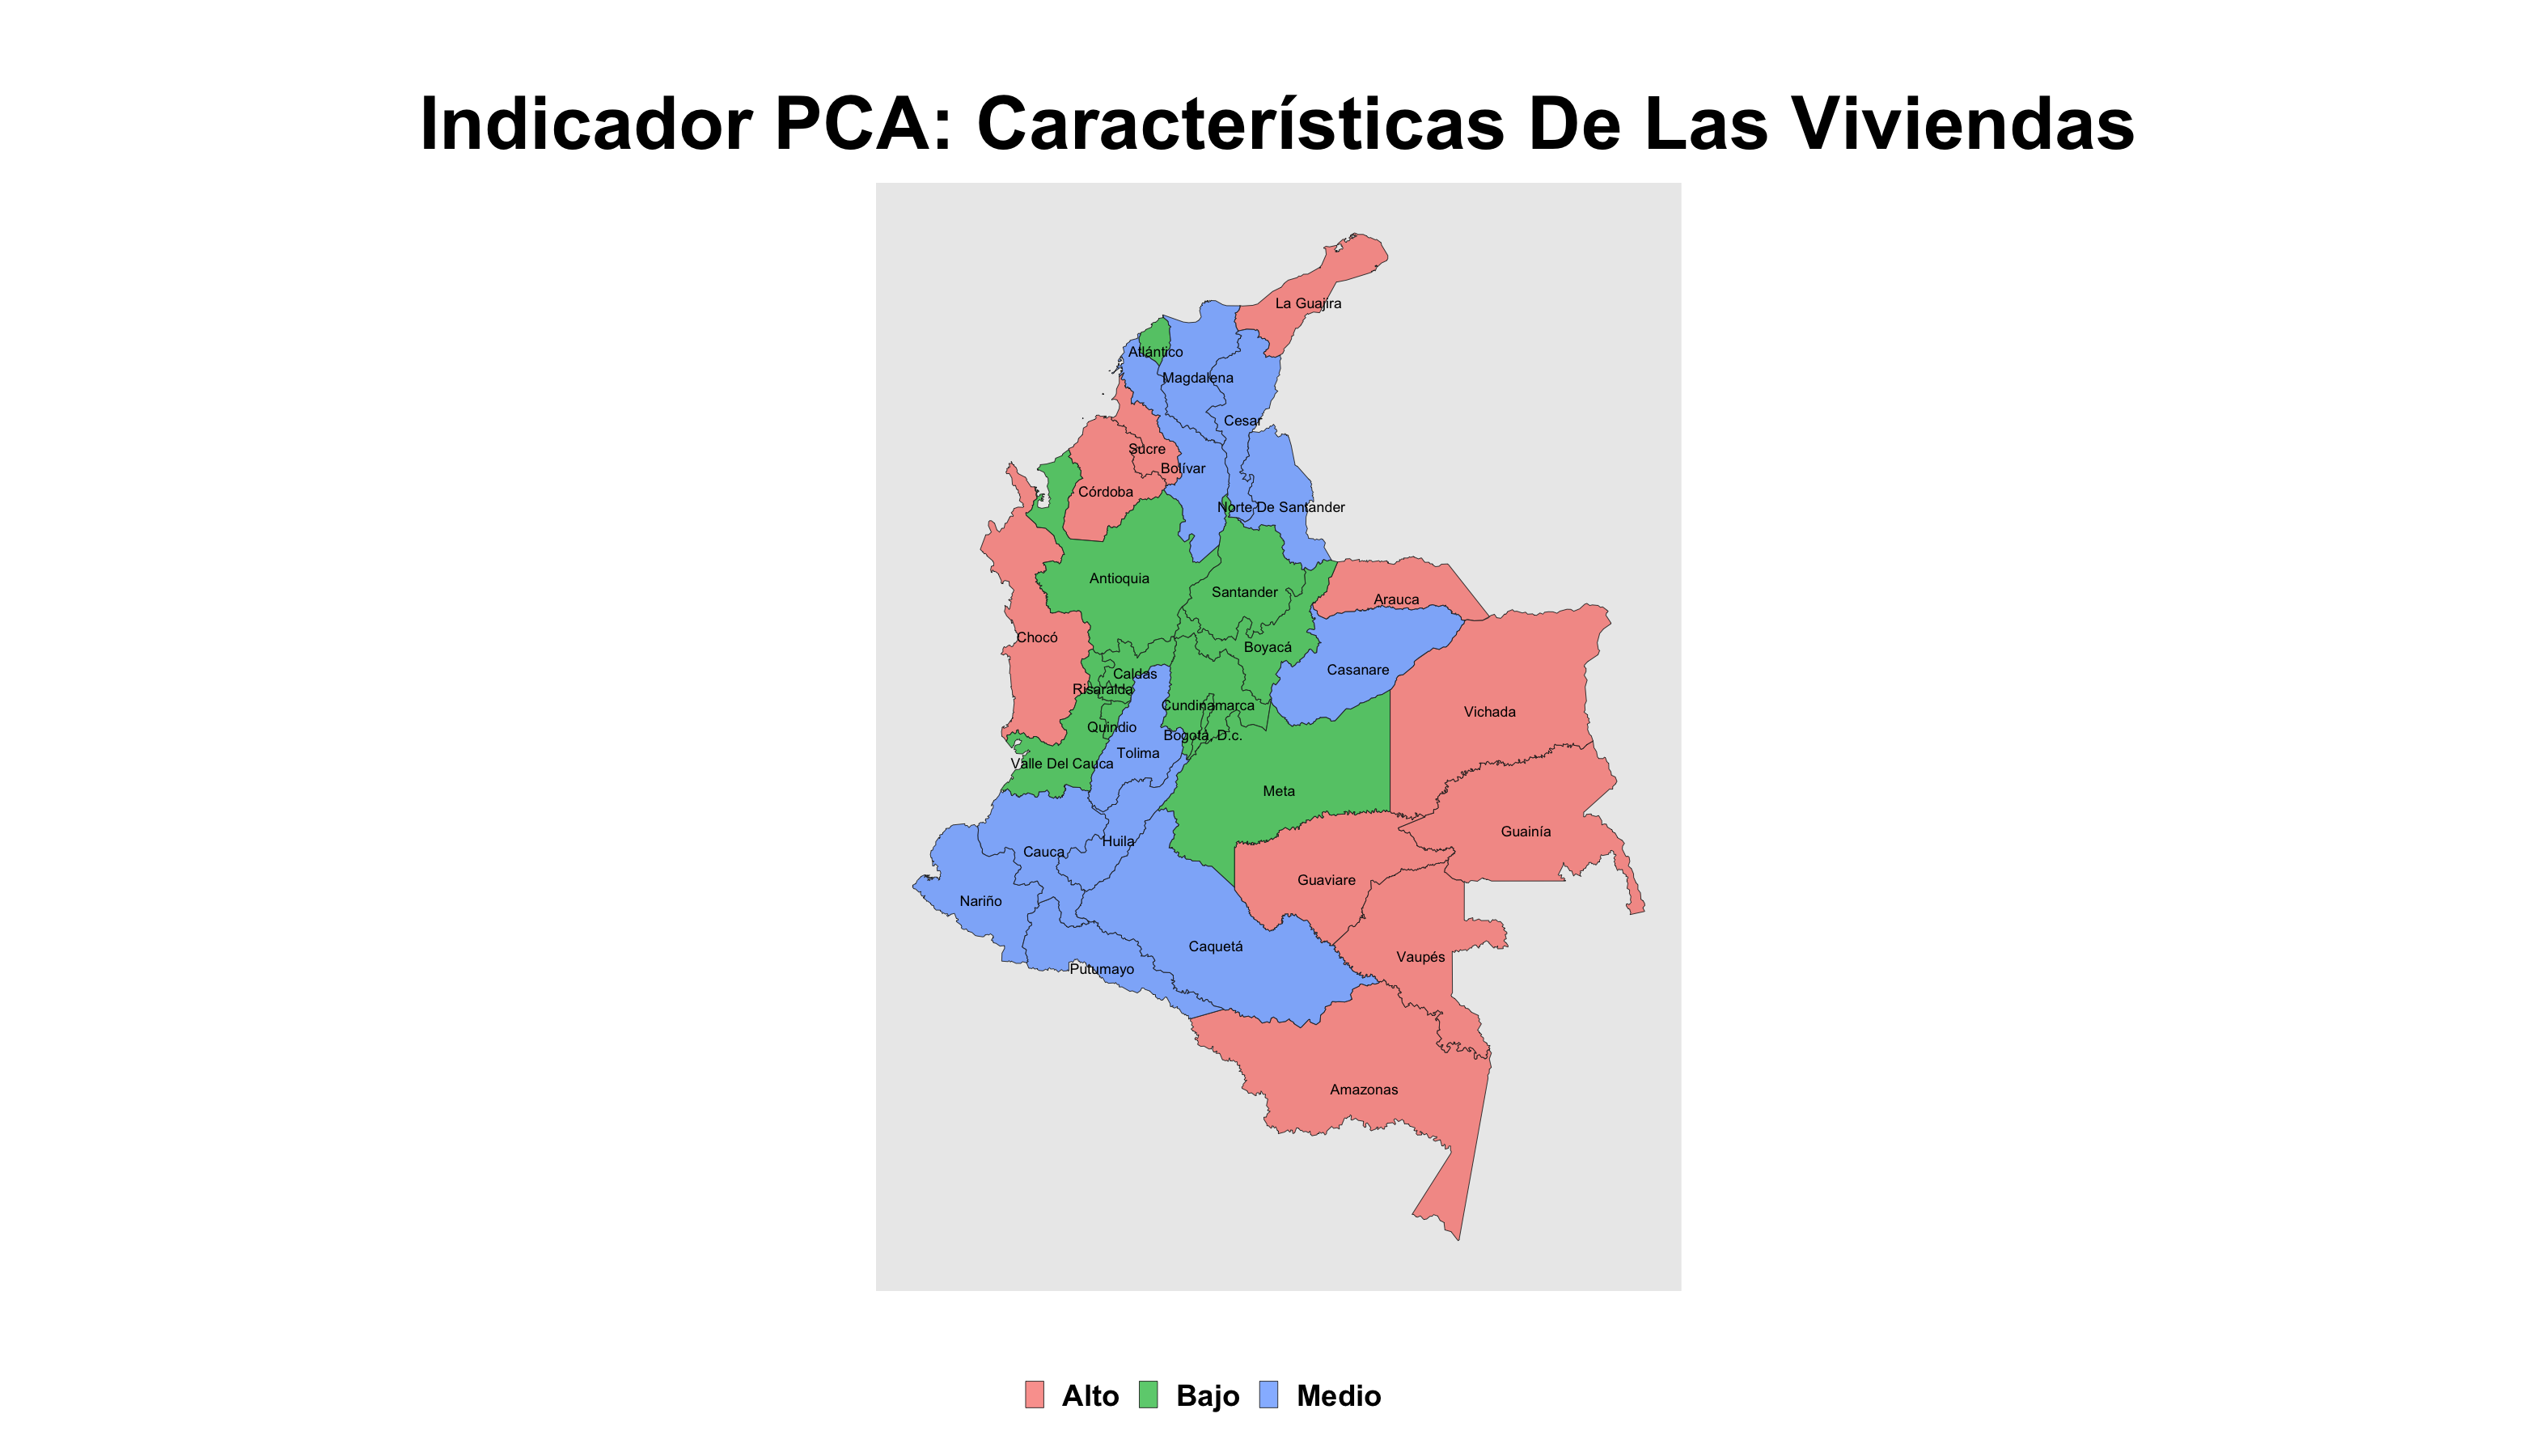
\includegraphics[width=\columnwidth]{img/pca_caracteristicas_de_las_viviendas_pca.png}
            \end{imagecolumn}
            \begin{textcolumn}
                \begin{itemize}
                    \item Existe una alta variación en el hacinamiento crítico entre regiones 
                    \item Esto puede estar asociado a las estructuras étnicas en algunos departamentos
                \end{itemize}
            \end{textcolumn}

    \printcolumns
    \end{slide}
    
    
       
    %%% ----------------------------
    %%% Características del hogar
    %%% ----------------------------
    \subsection{Crecimiento Económico}
    
        %%%-- Diversidad económica 
    \begin{slide}{8} 
                      \begin{imagecolumn}
                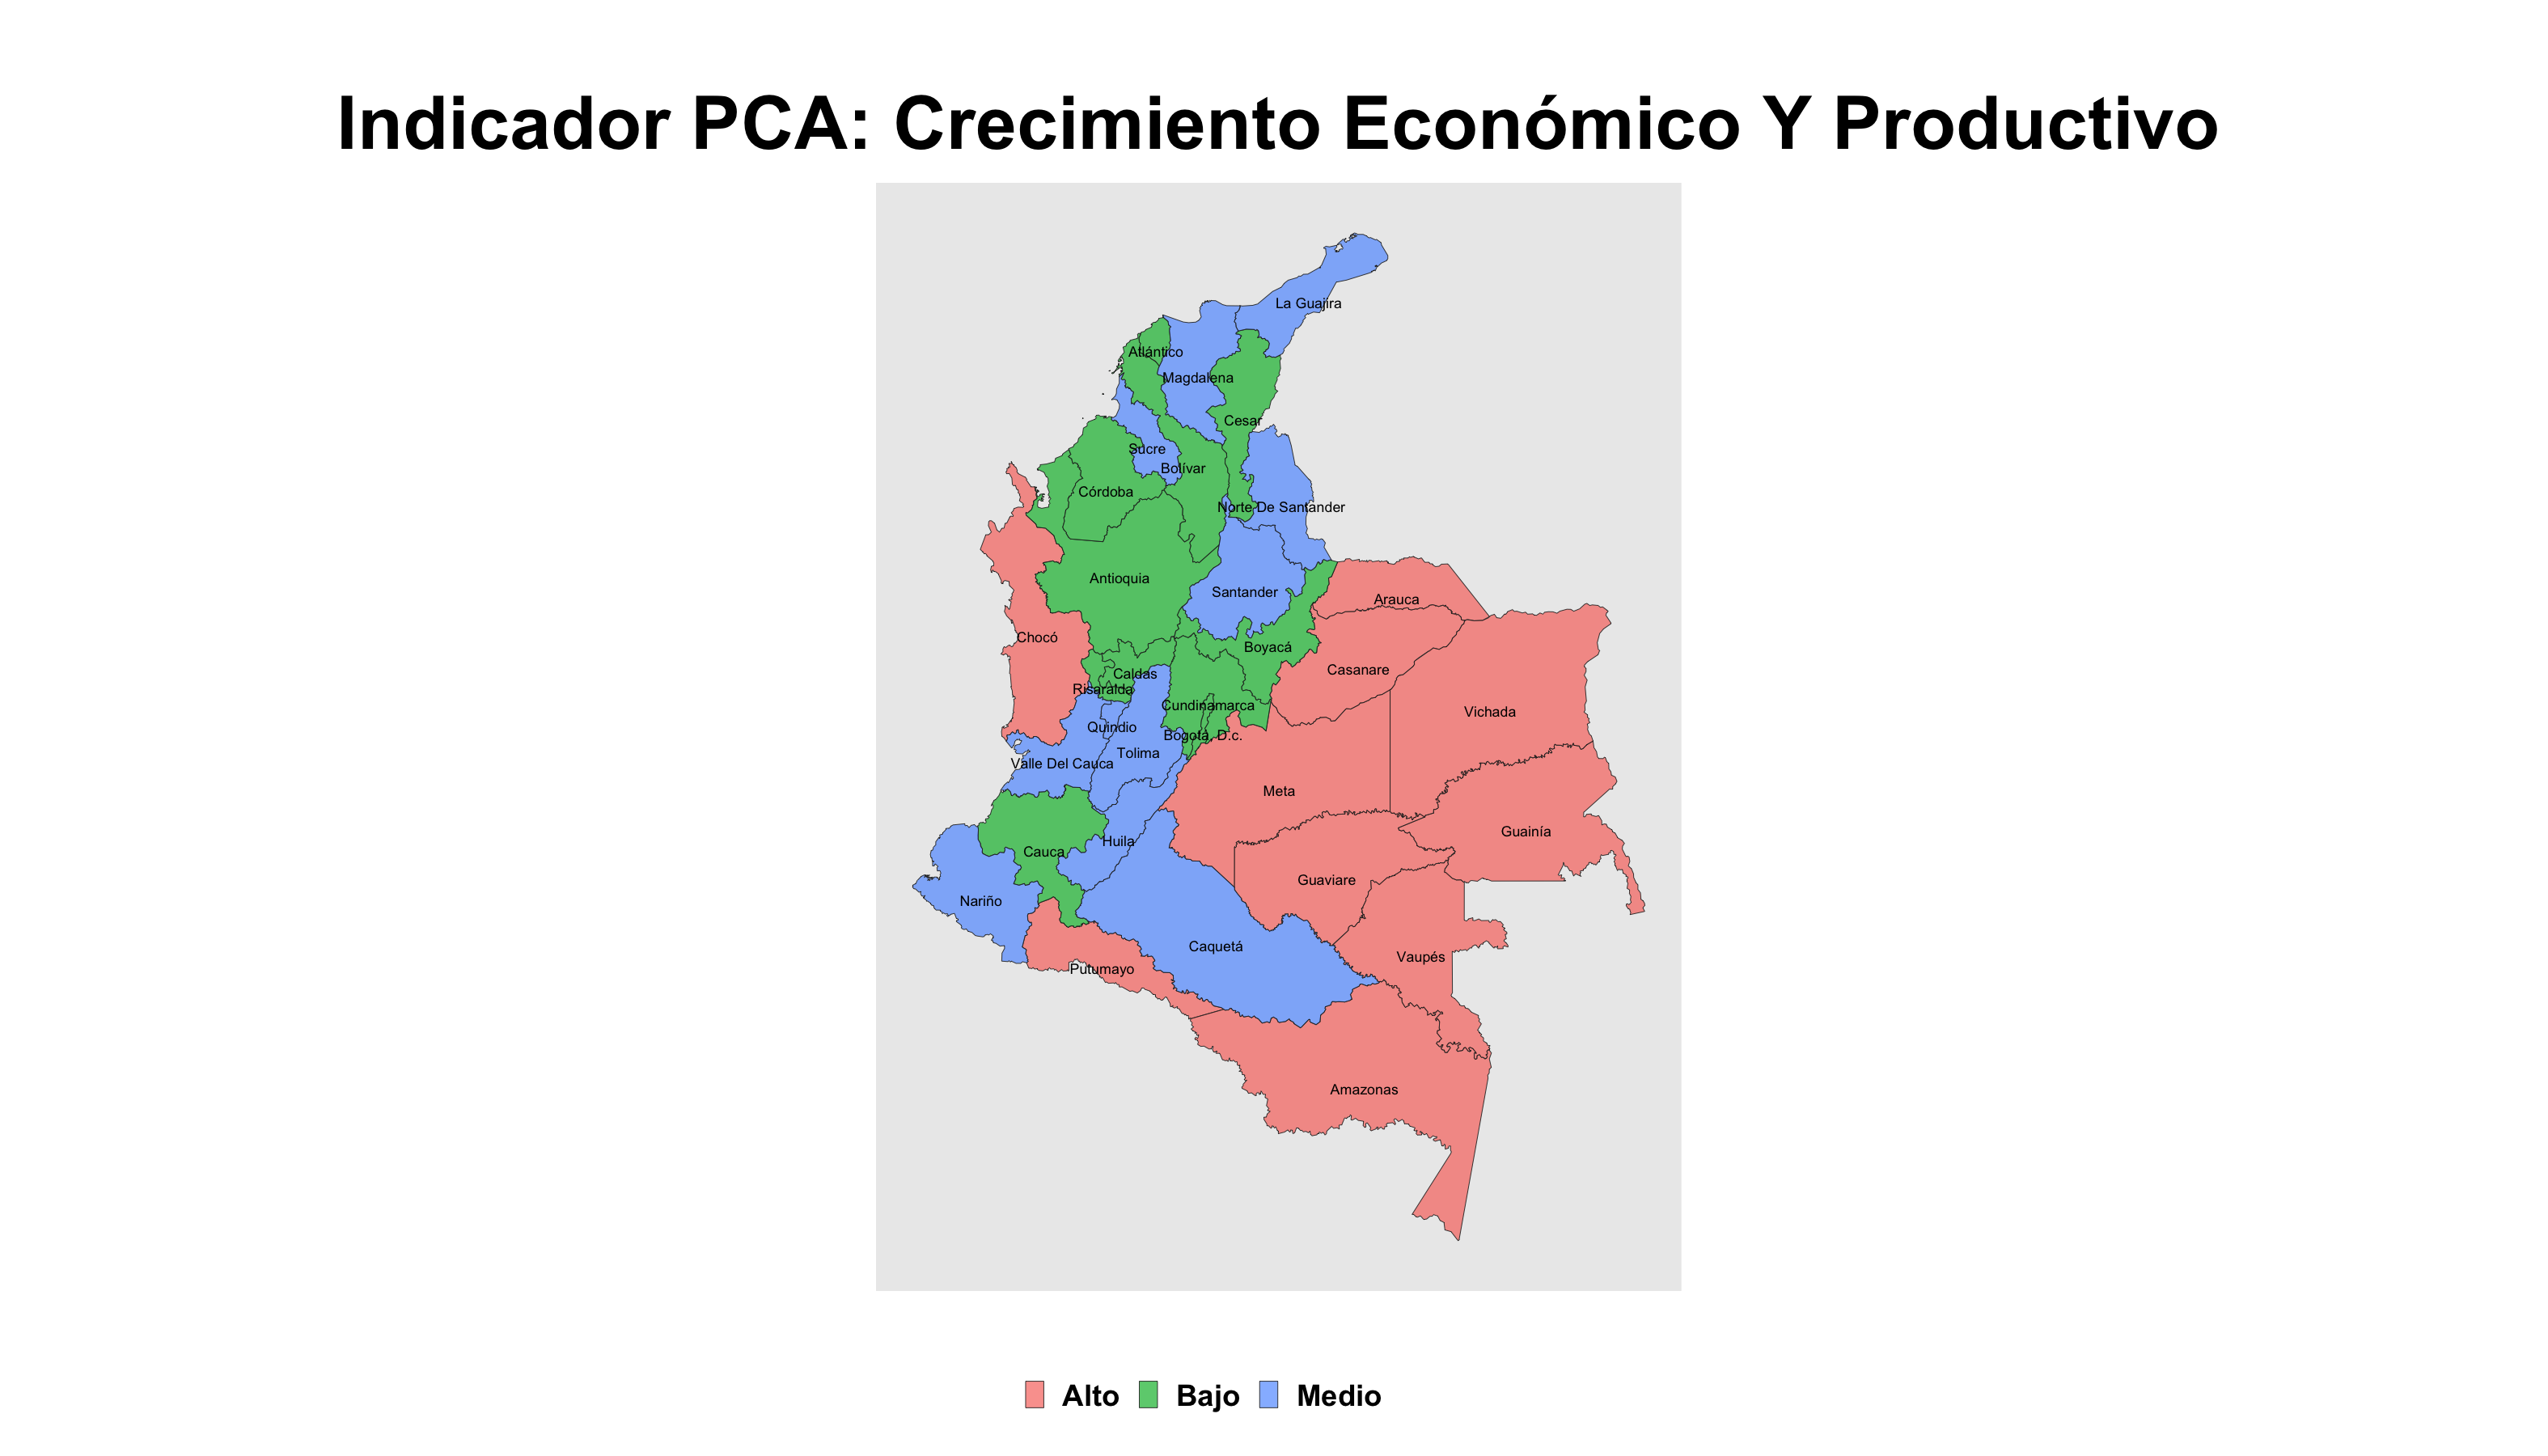
\includegraphics[width=\columnwidth]{img/pca_crecimiento_economico_y_productivo_pca.png}
            \end{imagecolumn}
            \begin{textcolumn}
                \begin{itemize}
                    \item Las regiones son ahora más diversas en términos de actividad económica.
                    \item Pero en los departamentos más marginados persiste una alta dependencia de ciertos sectores
                \end{itemize}
            \end{textcolumn}

    \printcolumns
    \end{slide}
    
    
    %%% ----------------------------
    %%% Migracion
    %%% ----------------------------
   
    
    %%% ----------------------------
    %%% Cambio Climático
    %%% ----------------------------
    \subsection{Cambio Climático}
    
        %%%-- Highlights 
    \begin{slide}{11} 
                      \begin{imagecolumn}
                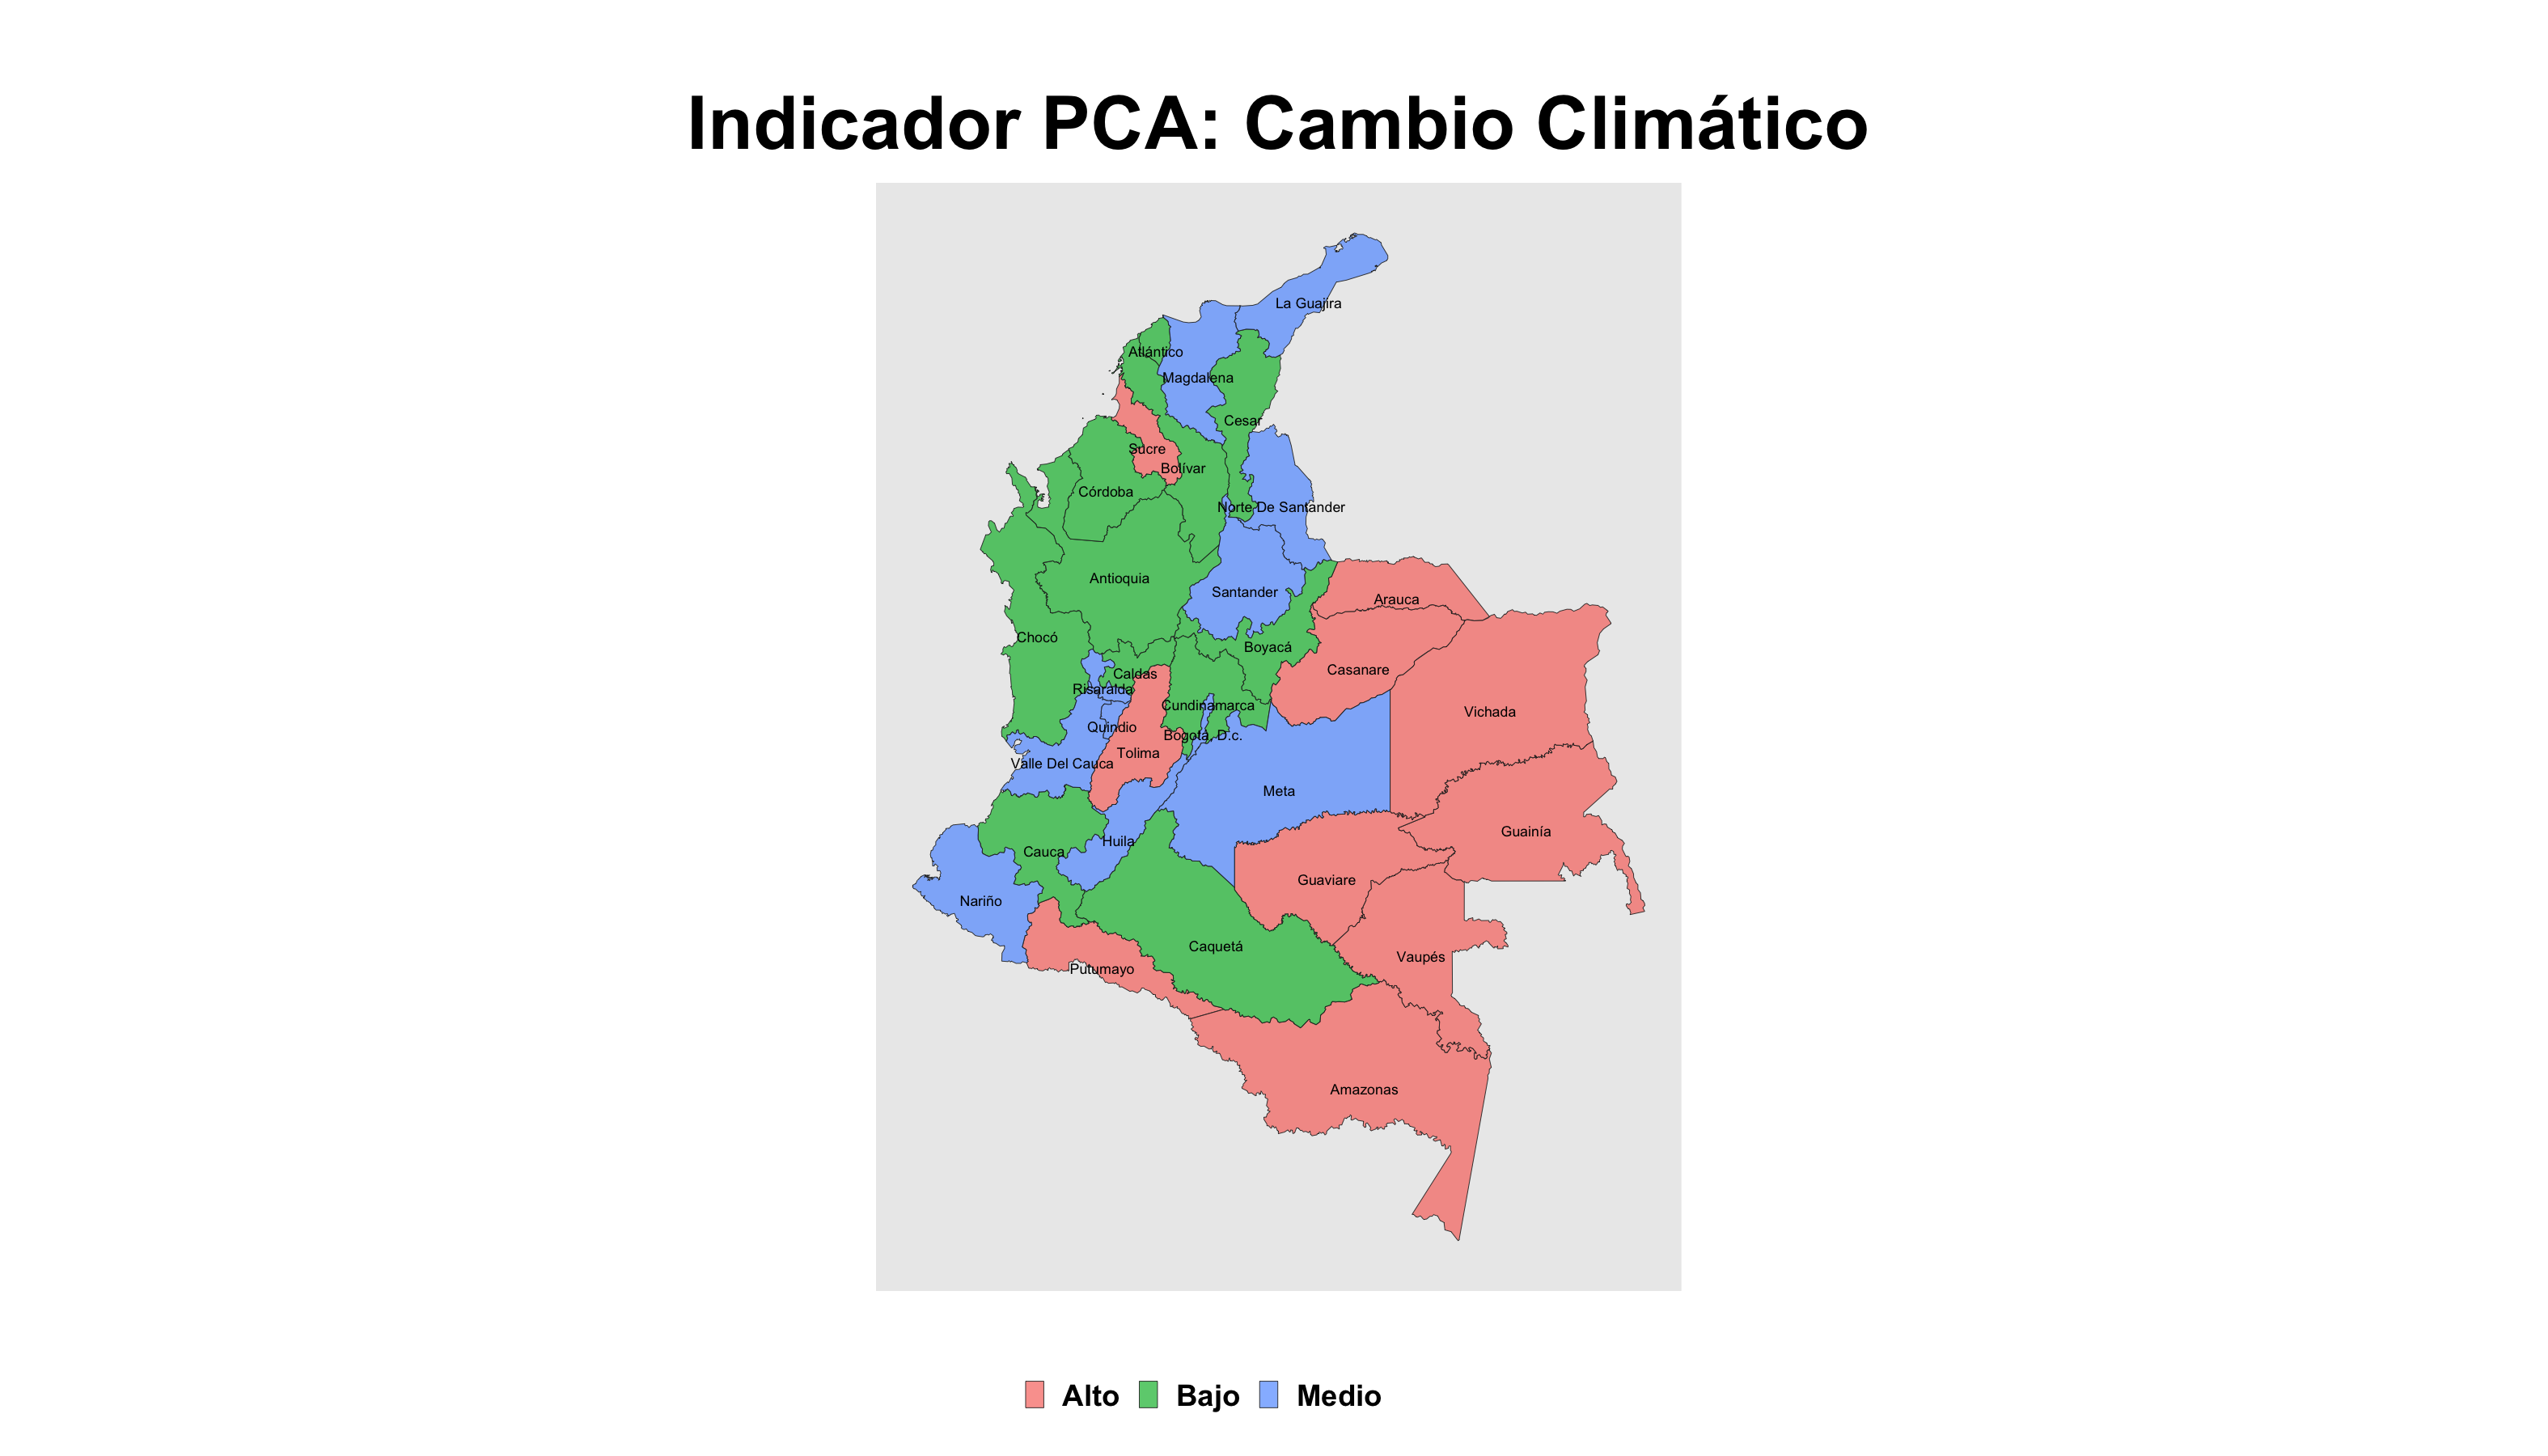
\includegraphics[width=\columnwidth]{img/pca_cambio_climatico_pca.png}
            \end{imagecolumn}
            \begin{textcolumn}
                \begin{itemize}
                    \item El impacto del cambio climático tendrá efectos diferenciados en las regiones del país
                \end{itemize}
            \end{textcolumn}

    \printcolumns
    \end{slide}
    
        %%% ----------------------------
    %%% Cambio Climático
    %%% ----------------------------
    \subsection{Covid}
    
        %%%-- Highlights 
    \begin{slide}{11} 
                      \begin{imagecolumn}
                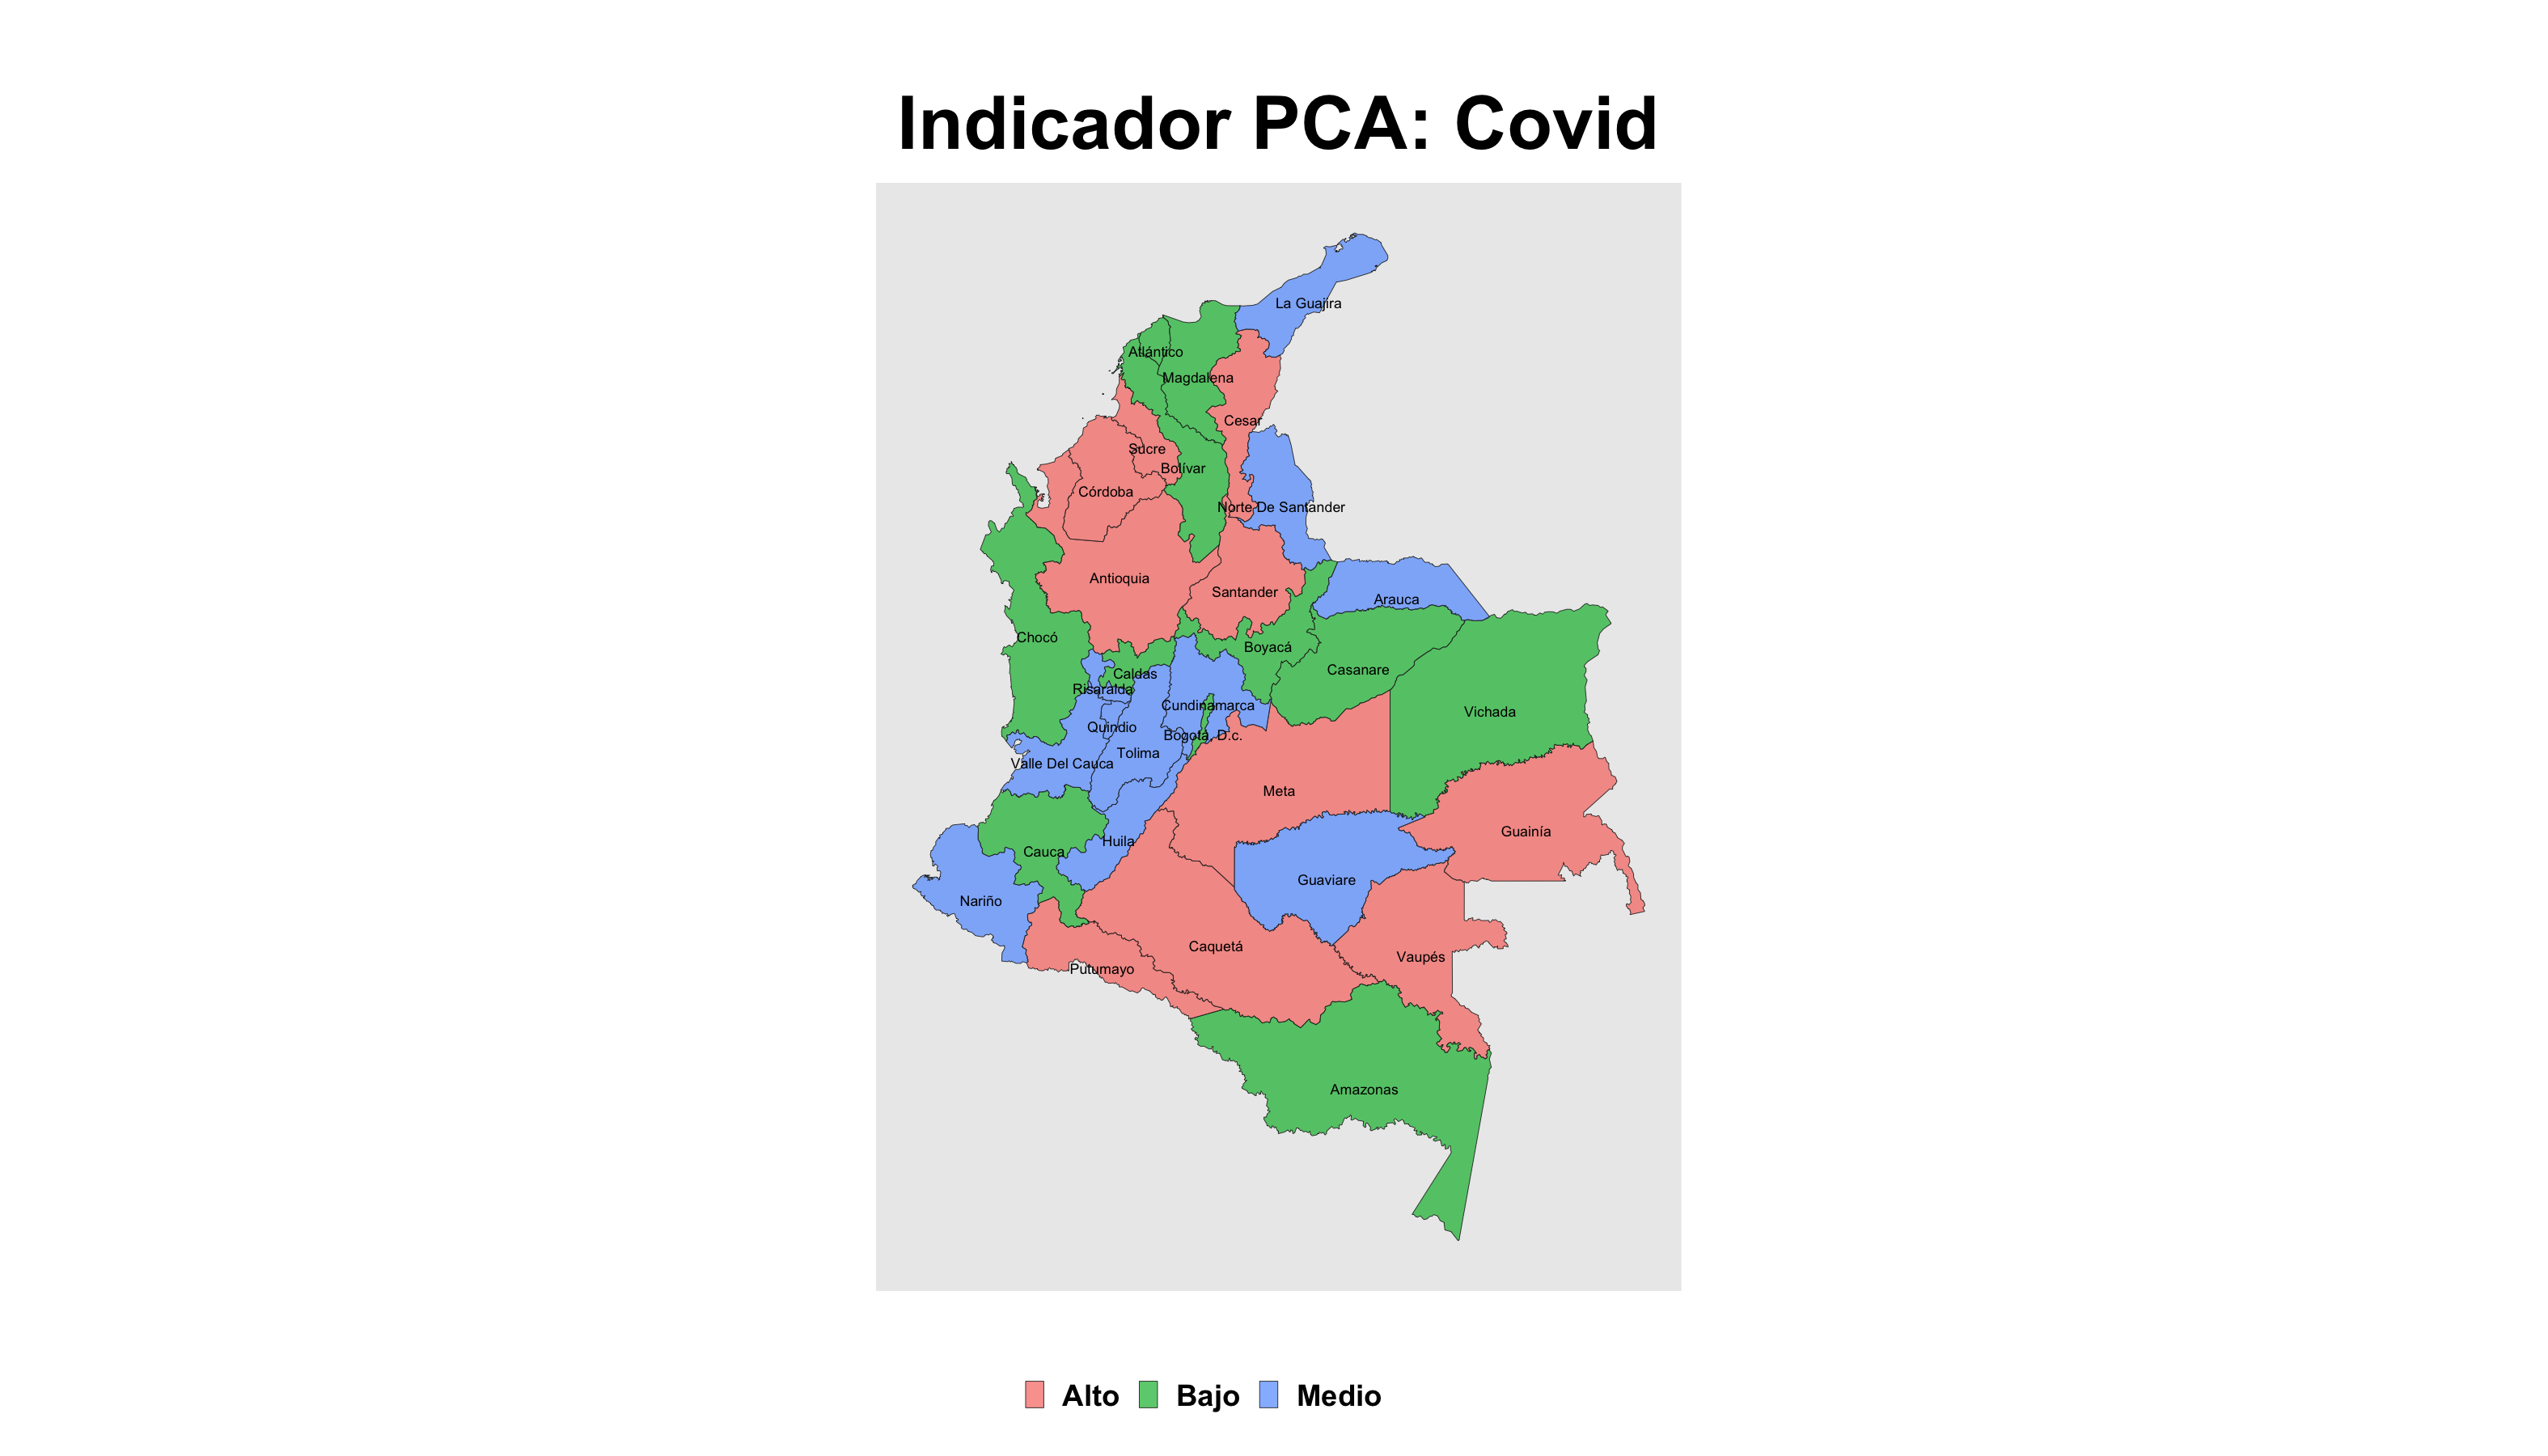
\includegraphics[width=\columnwidth]{img/pca_covid_pca.png}
            \end{imagecolumn}
            \begin{textcolumn}
                \begin{itemize}
                    \item El impacto del cambio climático tendrá efectos diferenciados en las regiones del país
                \end{itemize}
            \end{textcolumn}

    \printcolumns
    \end{slide}
    
        %%% ----------------------------
    %%% Indicadores de resutlados
    %%% ----------------------------
    
     \section{Resultados}
    %%% Contexto
    \slidetitle{12}
    
        %%% ----------------------------
    %%% Infancia y Niñez
    %%% ----------------------------
    \subsection{Infancia y niñez}
    
        %%%-- Tasa de Mortalidad Infantil 
    \begin{slide}{13} 
                      \begin{imagecolumn}
                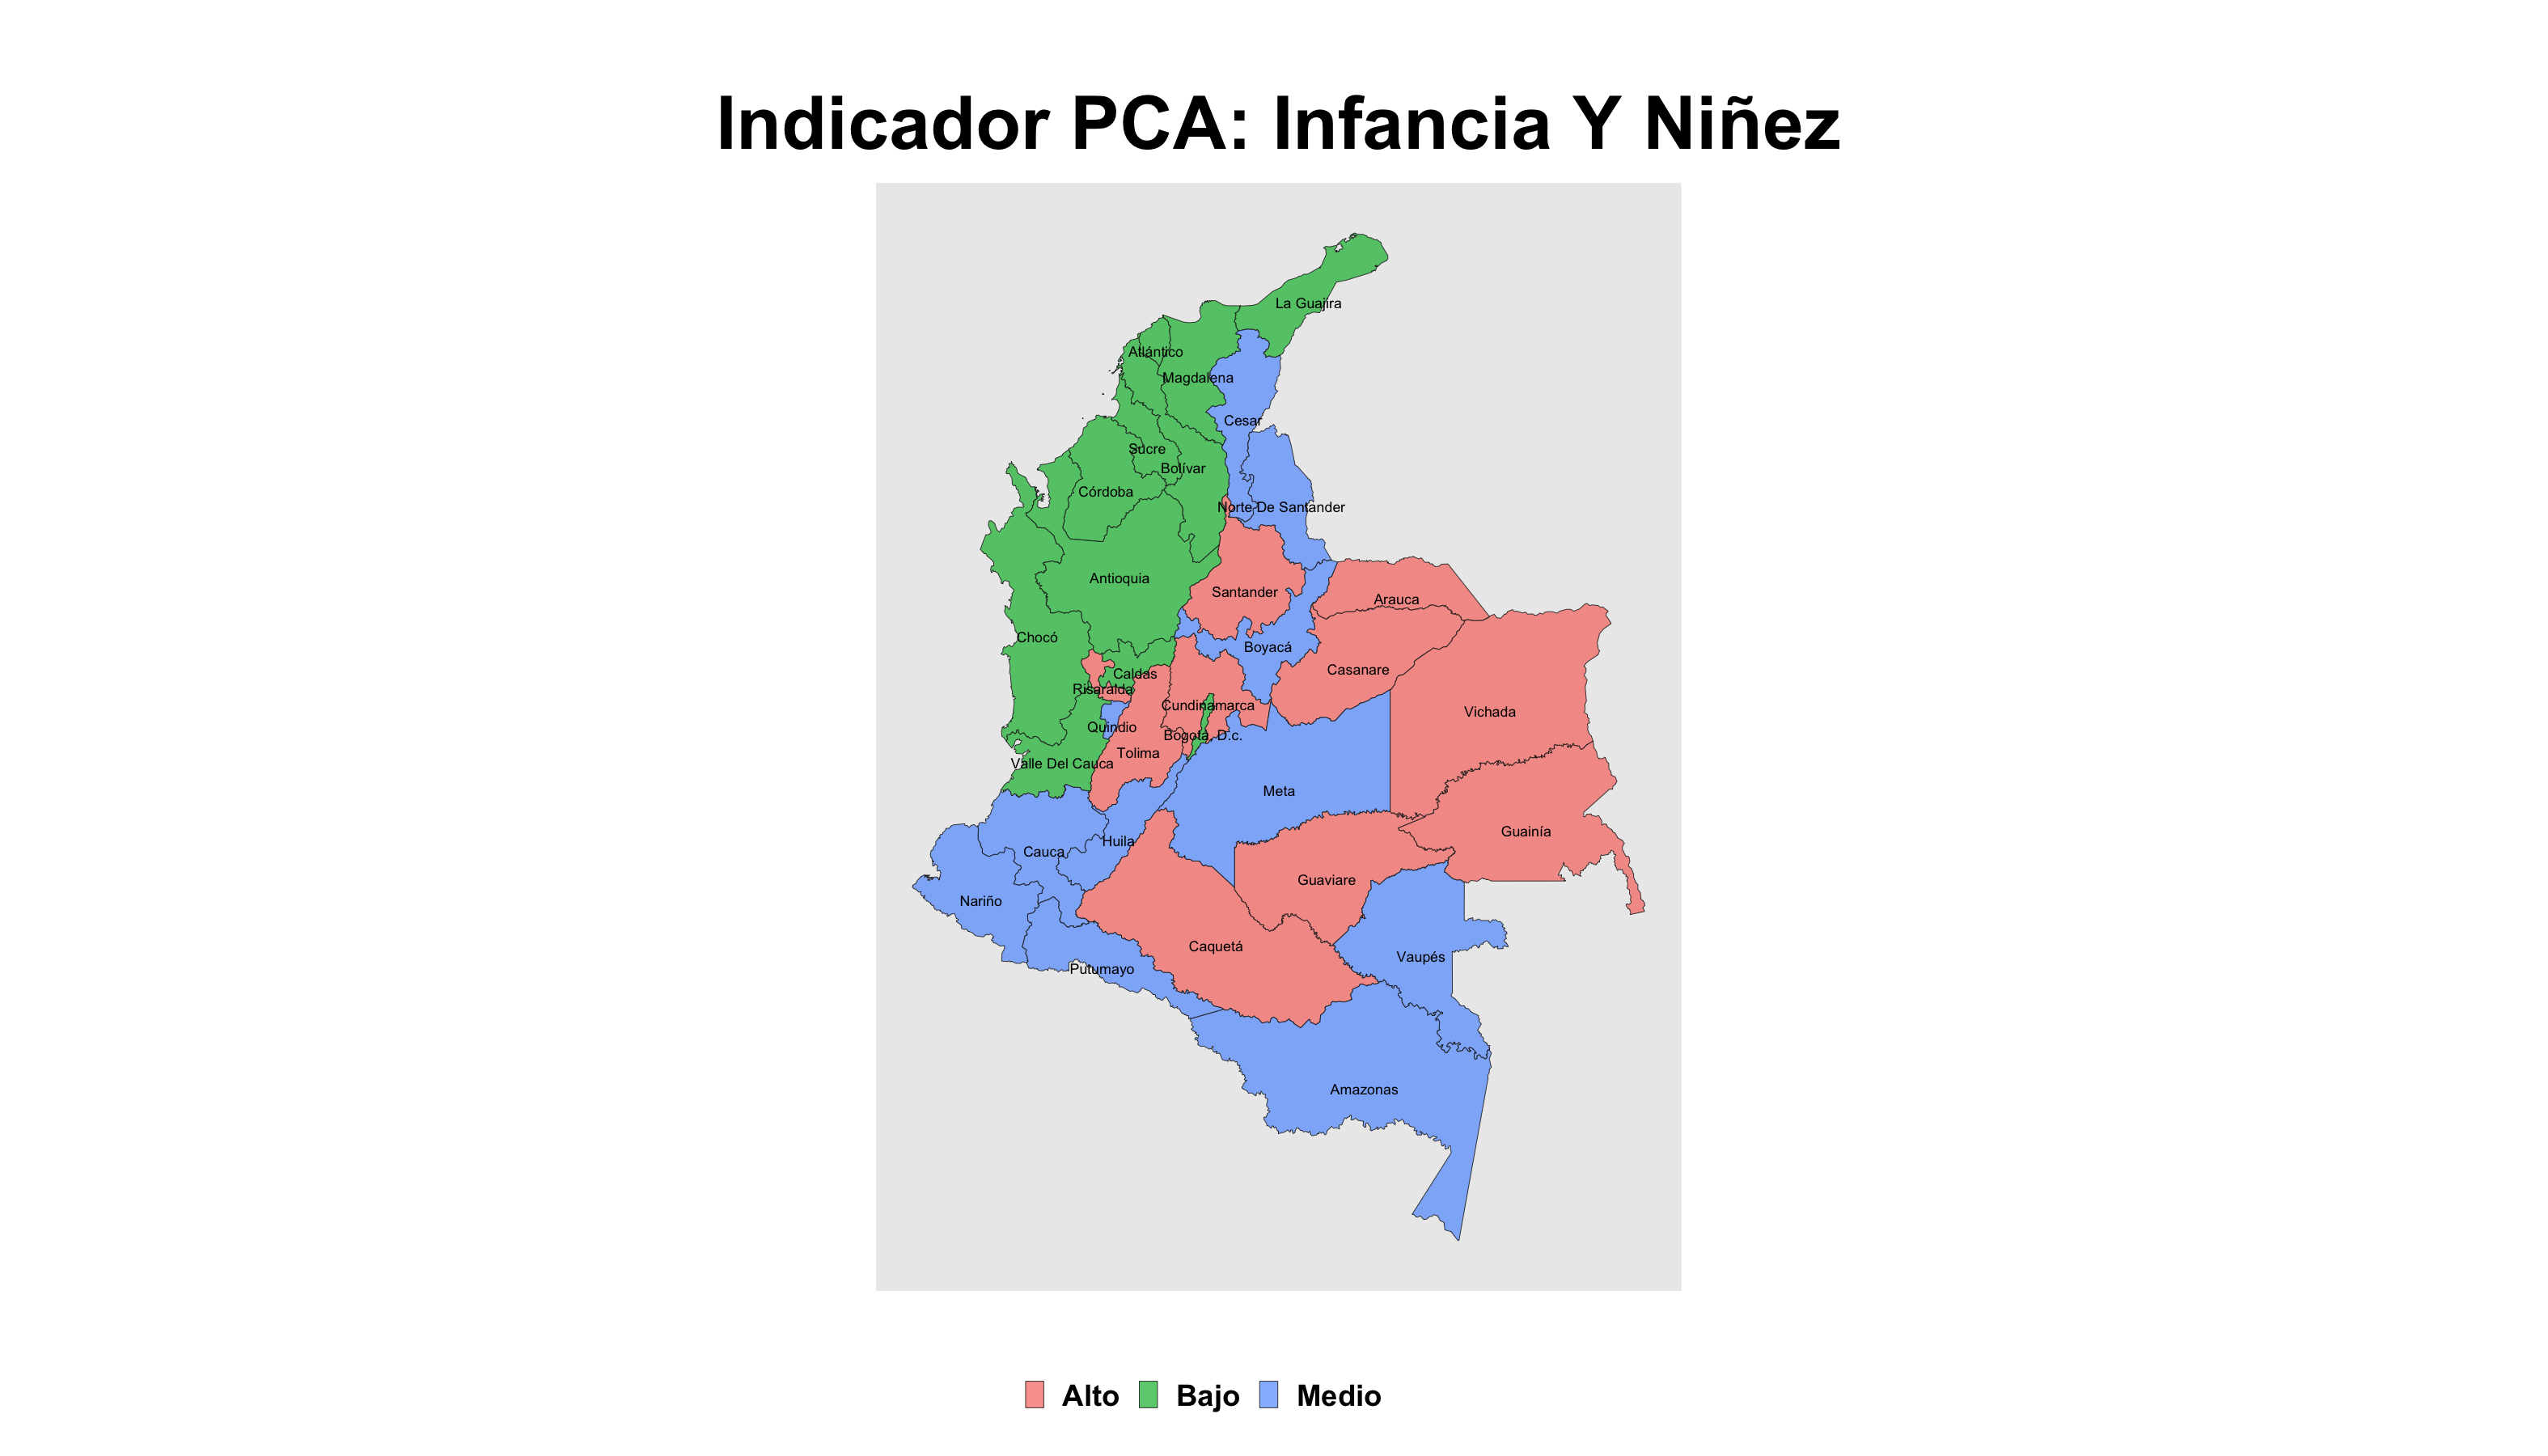
\includegraphics[width=\columnwidth]{img/pca_infancia_y_ninez_pca.png}
            \end{imagecolumn}
            \begin{textcolumn}
                \begin{itemize}
                    \item En Colombia coexisten regiones con tasas de mortalidad infantil similares a las de Sur Africa (24%, Vichada) y a las de Estados Unidos (6%, Boyacá)
                \end{itemize}
            \end{textcolumn}

    \printcolumns
    \end{slide}
    
       
      %%% ----------------------------
    %%% Juventud
    %%% ----------------------------
    \subsection{Juventud}
    
    %%%-- Educación Superior
    \begin{slide}{14} 
                      \begin{imagecolumn}
                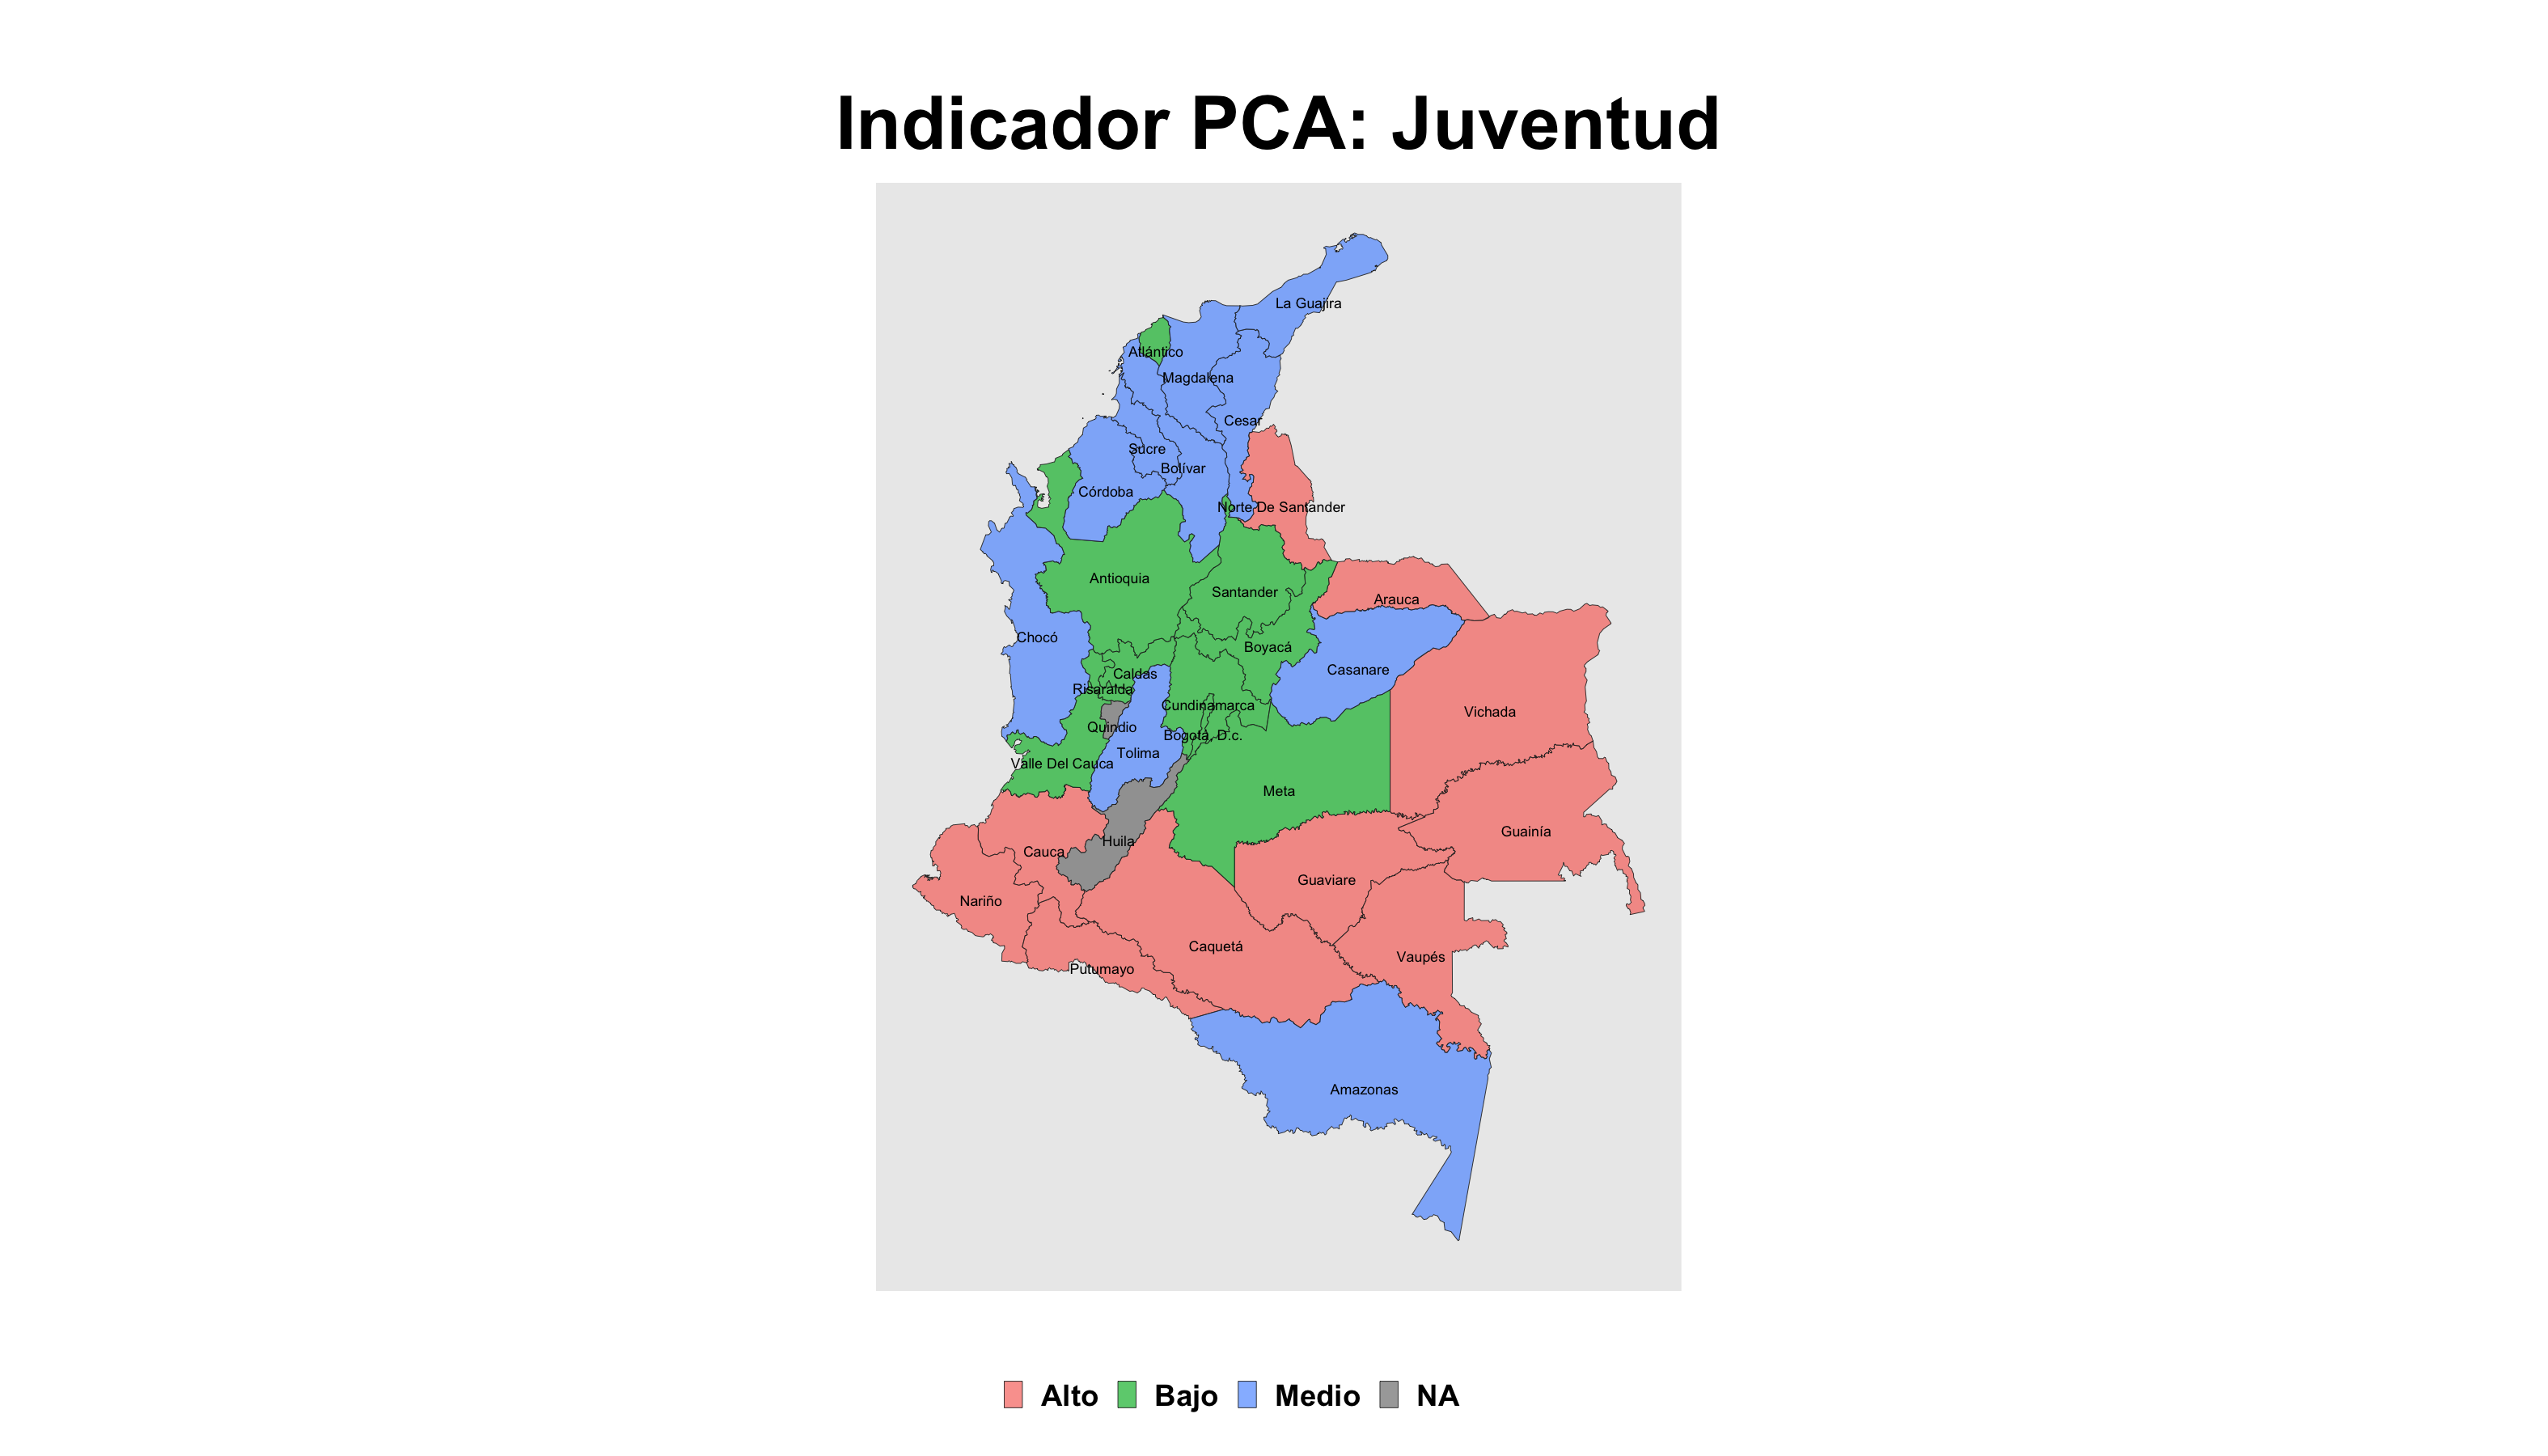
\includegraphics[width=\columnwidth]{img/pca_juventud_pca.png}
            \end{imagecolumn}
            \begin{textcolumn}
                \begin{itemize}
                    \item Existe una alta desigualdad en el acceso a la educación superior entre regiones
                    \item Mientras que en Bogotá el 43% de los jóvenes ha asistido a institutos de educación superior por al menos 1 año, en Vichada éste porcentaje es de sólo 7%
                    \item Éstas diferencias no han cambiado mucho en el tiempo 
                \end{itemize}
            \end{textcolumn}

    \printcolumns
    \end{slide}
    
      %%% ----------------------------
    %%% Cambio Climático
    %%% ----------------------------
    \subsection{Adultez}
    
            %%%-- Highlights 
    \begin{slide}{15} 
            \begin{imagecolumn}
                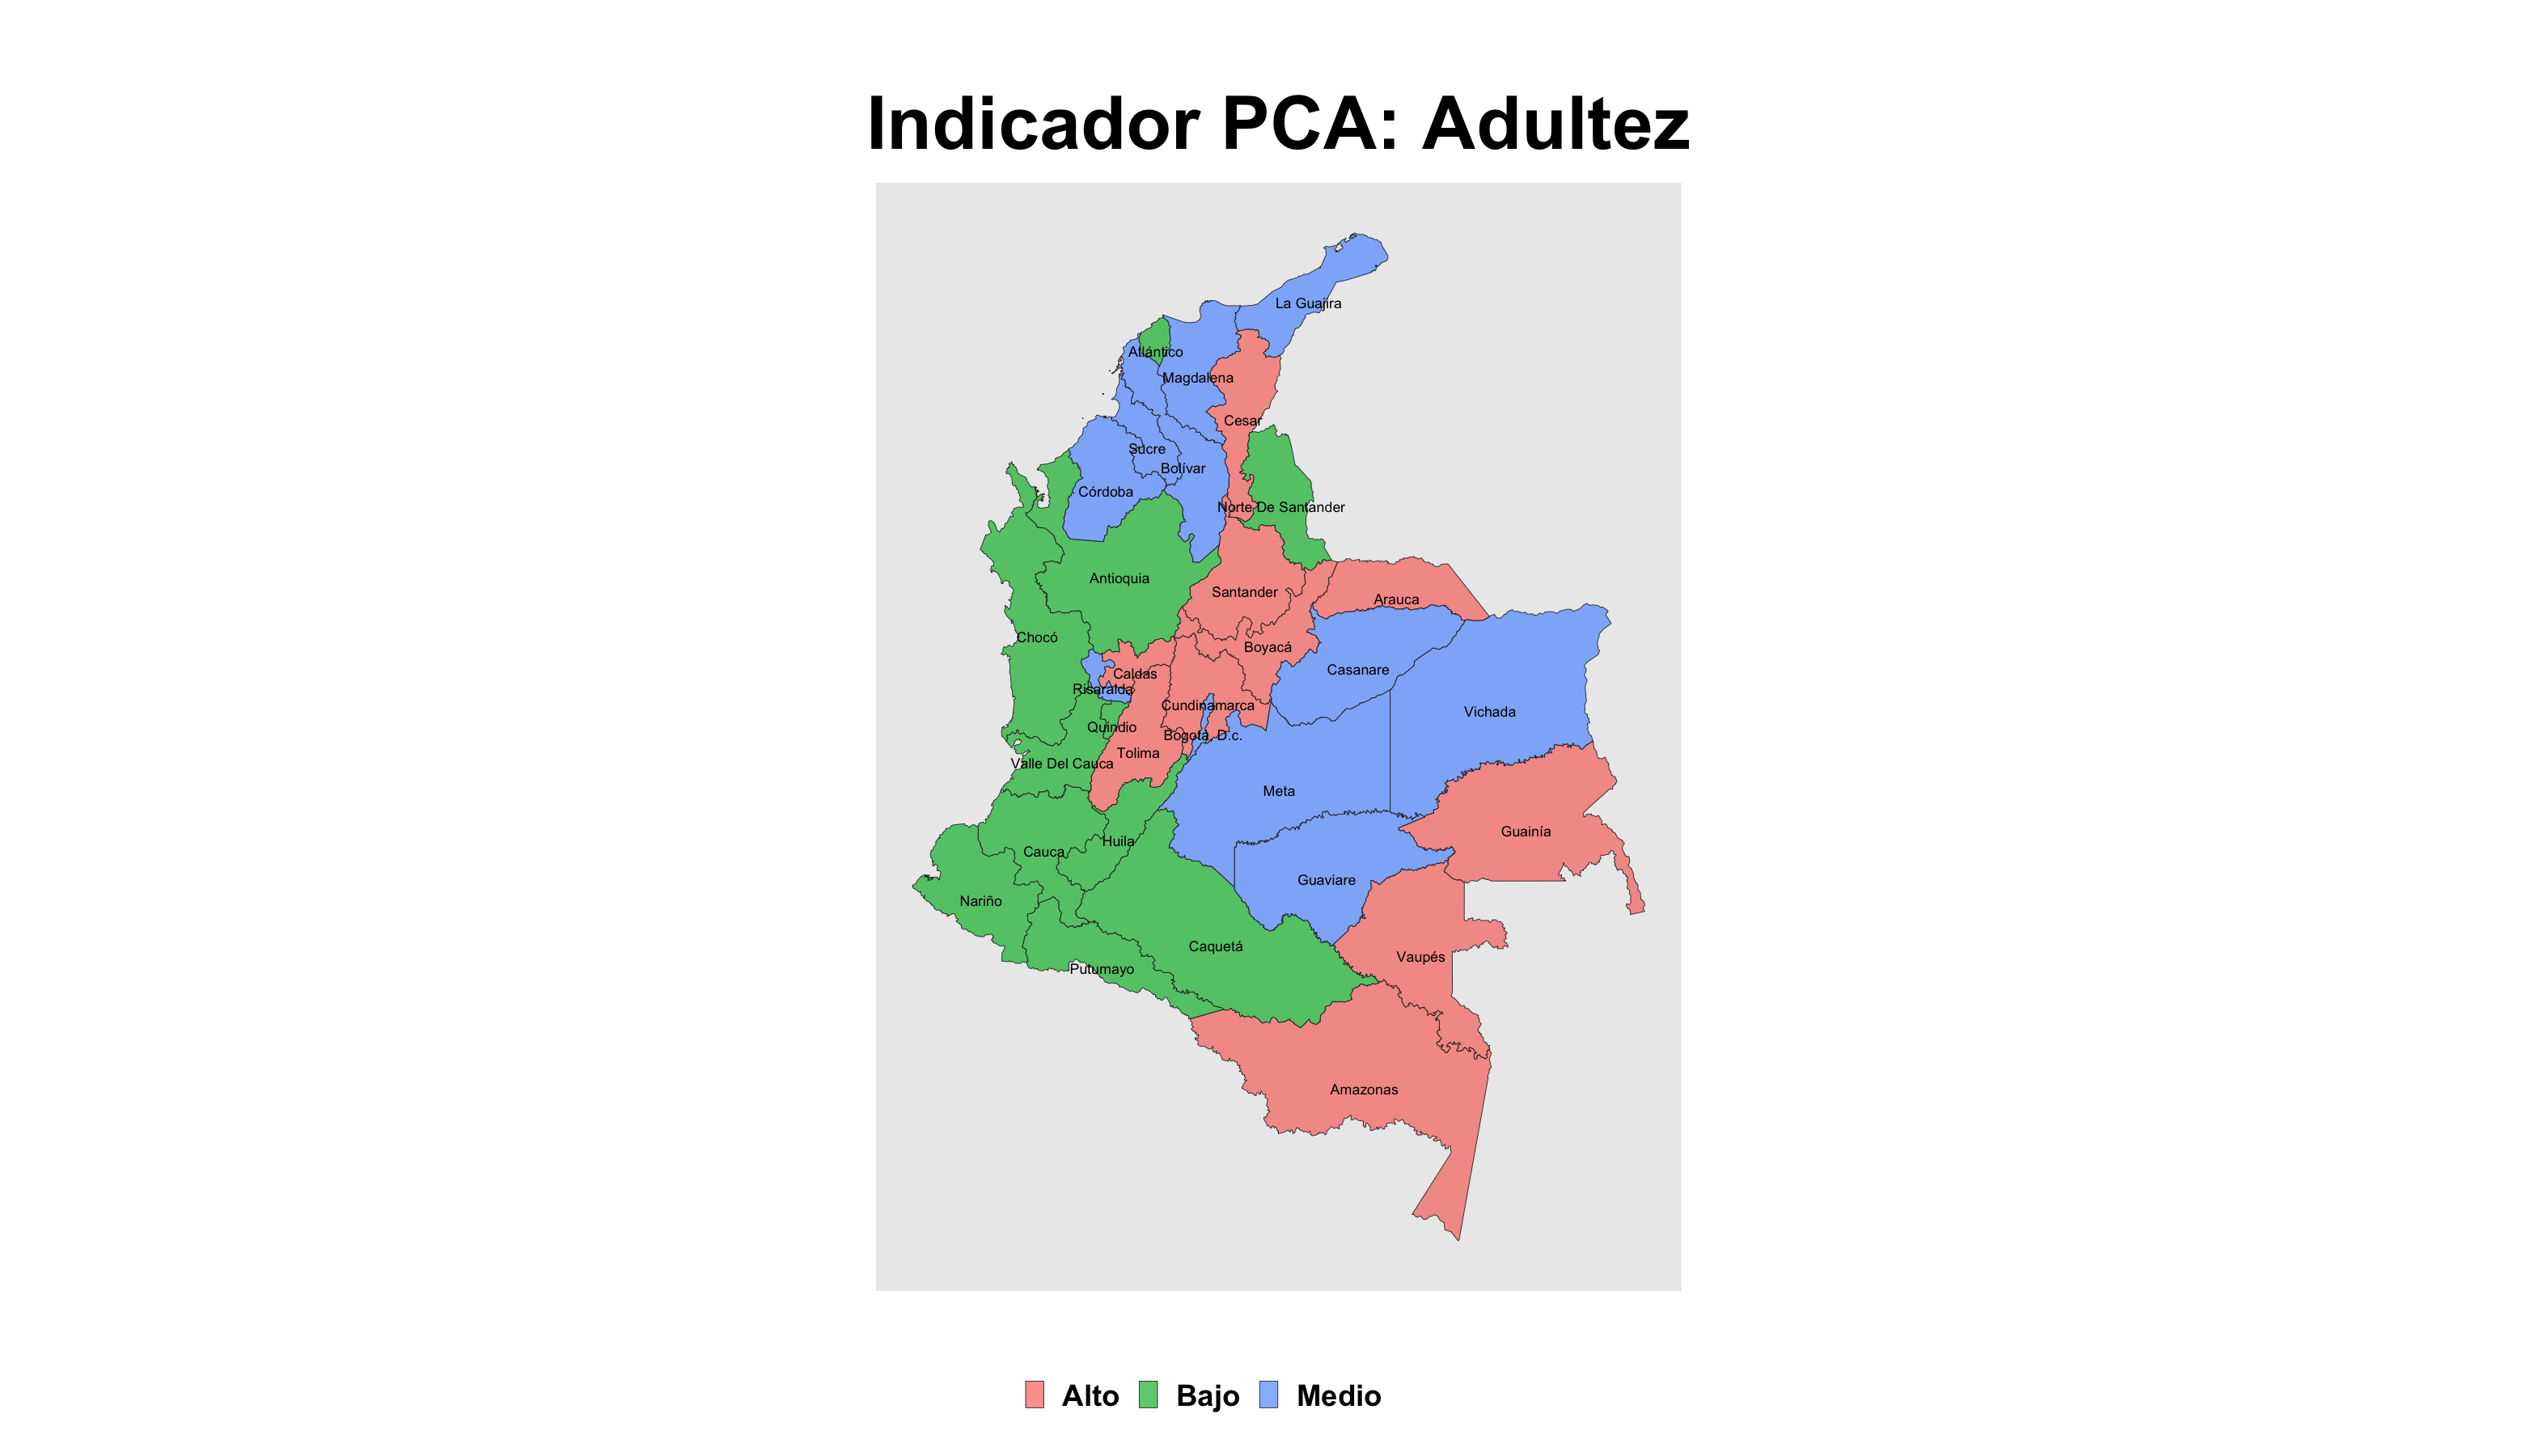
\includegraphics[width=\columnwidth]{img/pca_adultez_pca.png}
            \end{imagecolumn}
            \begin{textcolumn}
                \begin{itemize}
                    \item Un incremento en el desempleo generalizado debido a la pandemia
                    \item Con algunas ciudades donde se ha agudizado en mayor magnitud
                \end{itemize}
            \end{textcolumn}
    \printcolumns
    \end{slide}
    
    
    
      %%% ----------------------------
    %%% Cambio Climático
    %%% ----------------------------
    \subsection{Adultez}
    
            %%%-- Highlights 
    \begin{slide}{16} 
            \begin{imagecolumn}
                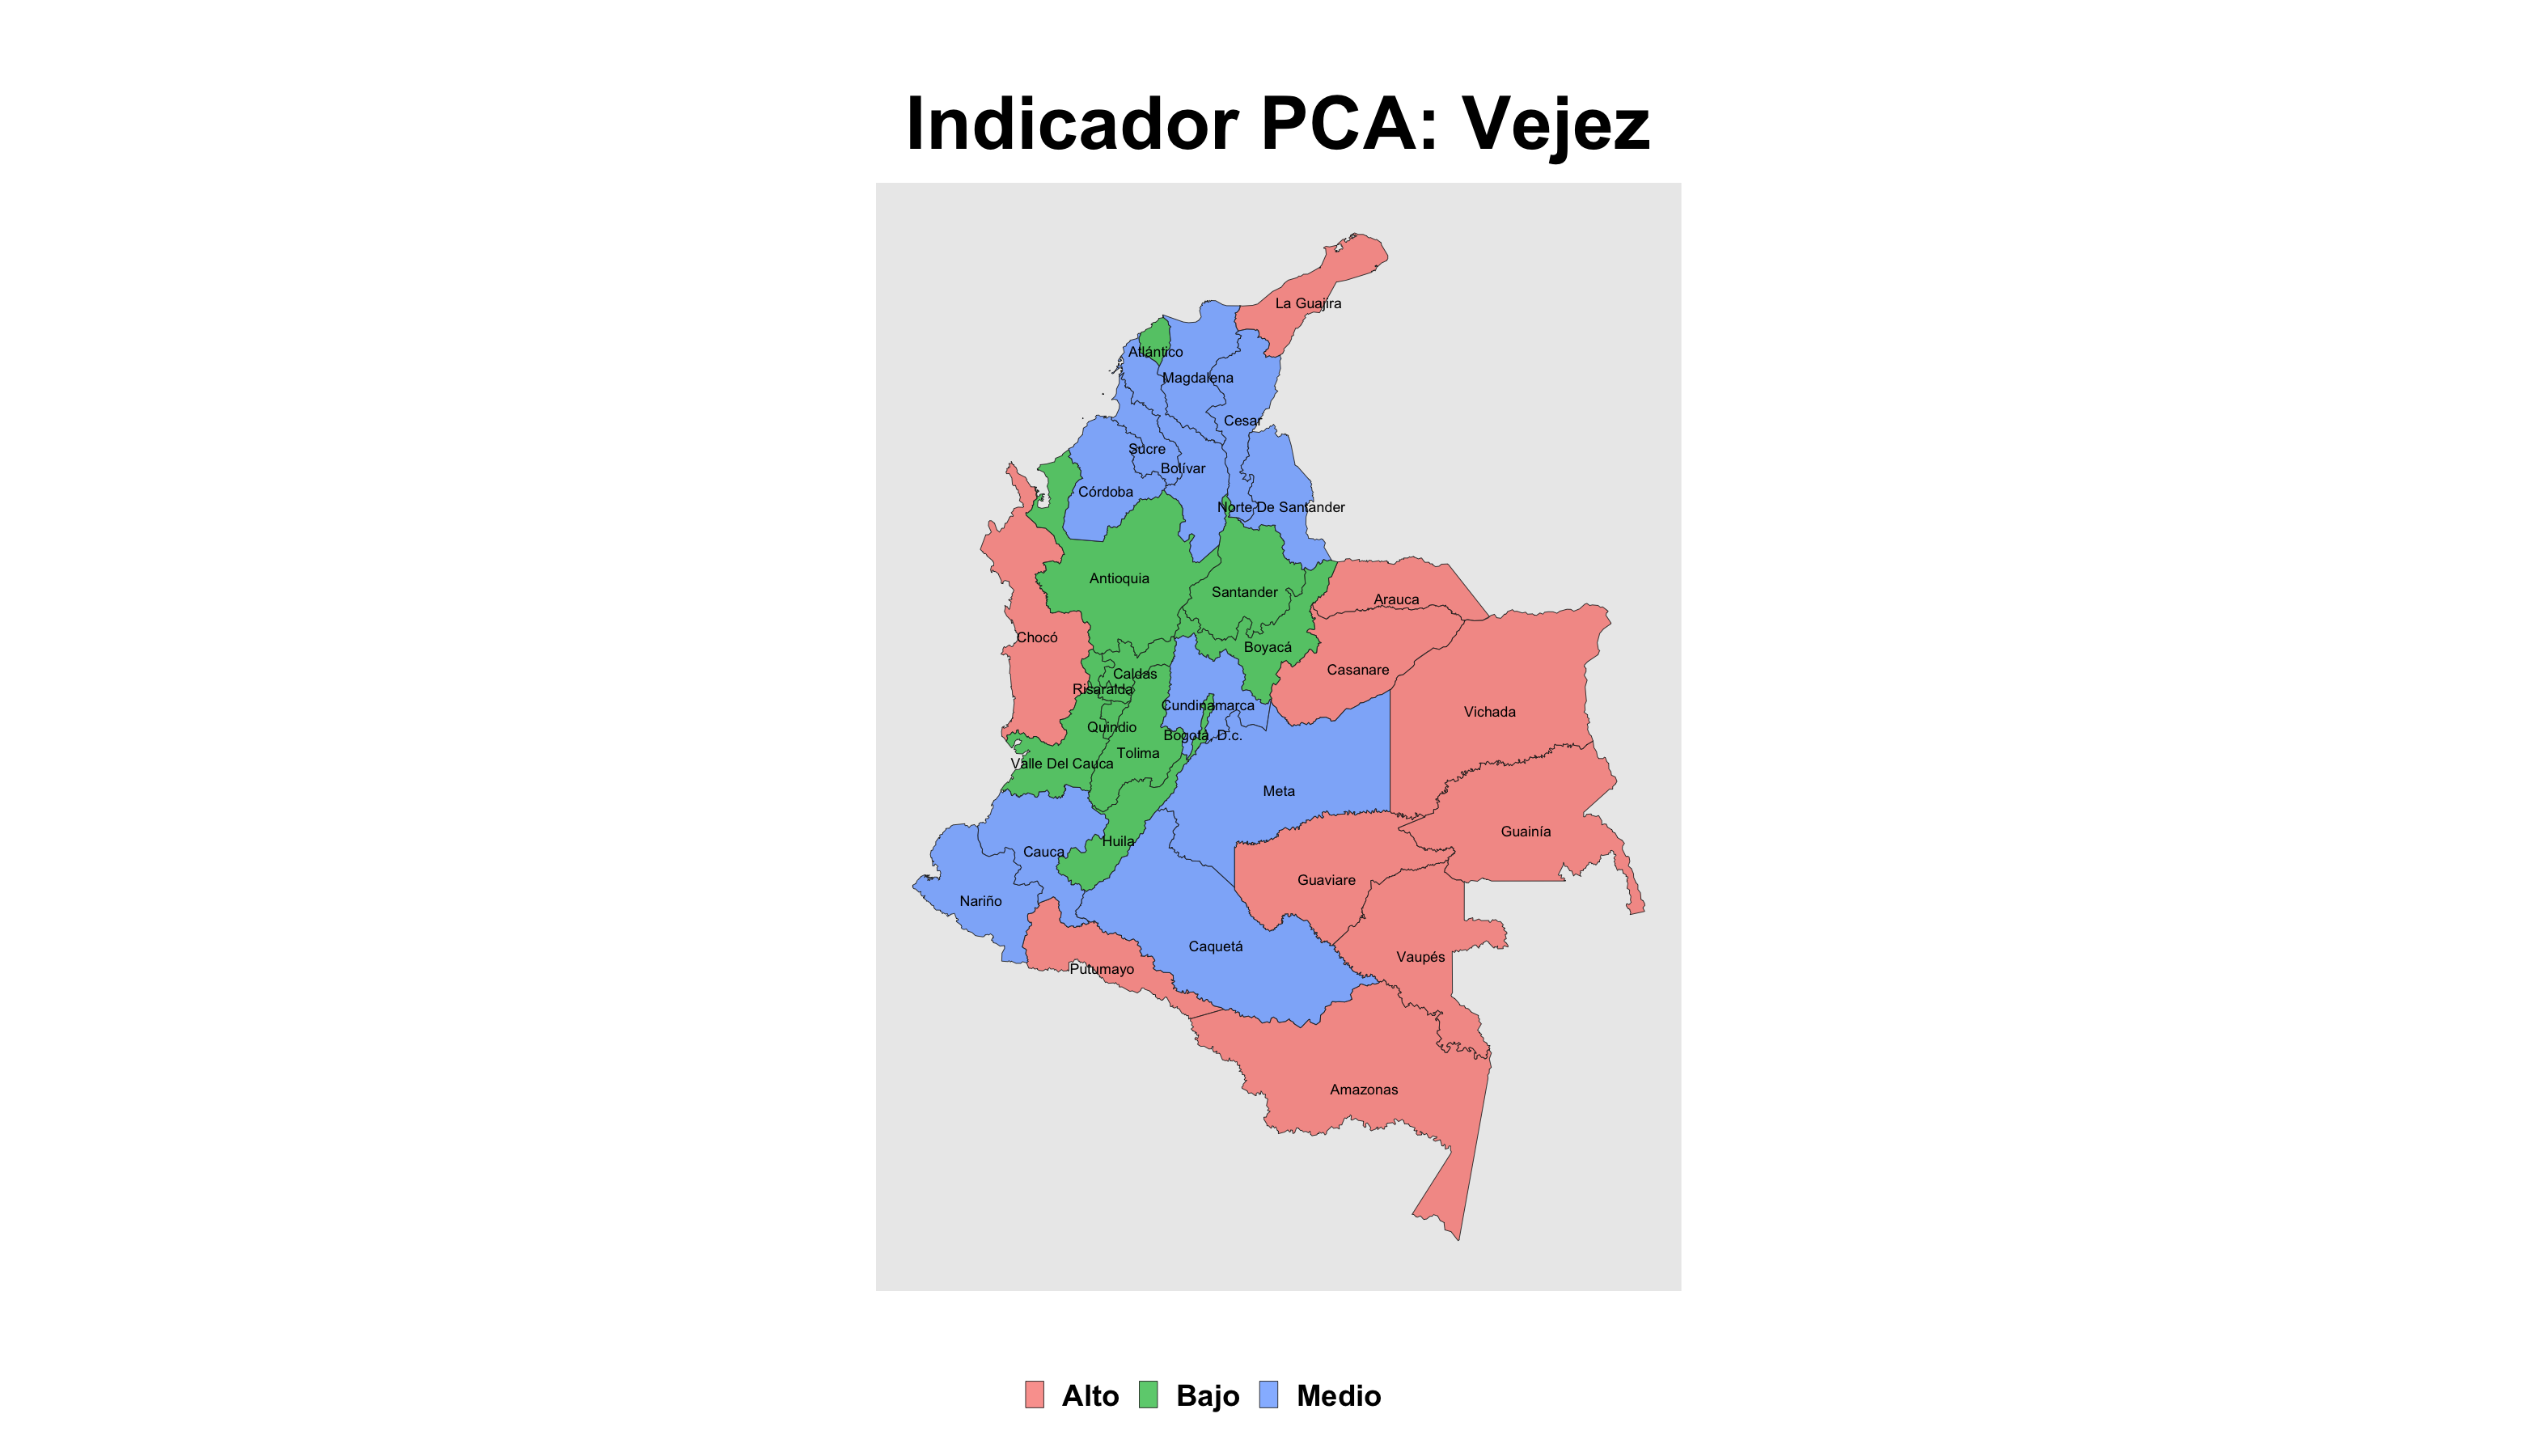
\includegraphics[width=\columnwidth]{img/pca_vejez_pca.png}
            \end{imagecolumn}
            \begin{textcolumn}
                \begin{itemize}
                    \item Un incremento en el desempleo generalizado debido a la pandemia
                    \item Con algunas ciudades donde se ha agudizado en mayor magnitud
                \end{itemize}
            \end{textcolumn}
    \printcolumns
    \end{slide}
    
          %%% ----------------------------
    %%% Cambio Climático
    %%% ----------------------------
      \section{Colombias}
    %%% Contexto
    \slidetitle{17}
    
                %%%-- Highlights 
    \begin{slide}{18} 
            \begin{imagecolumn}
                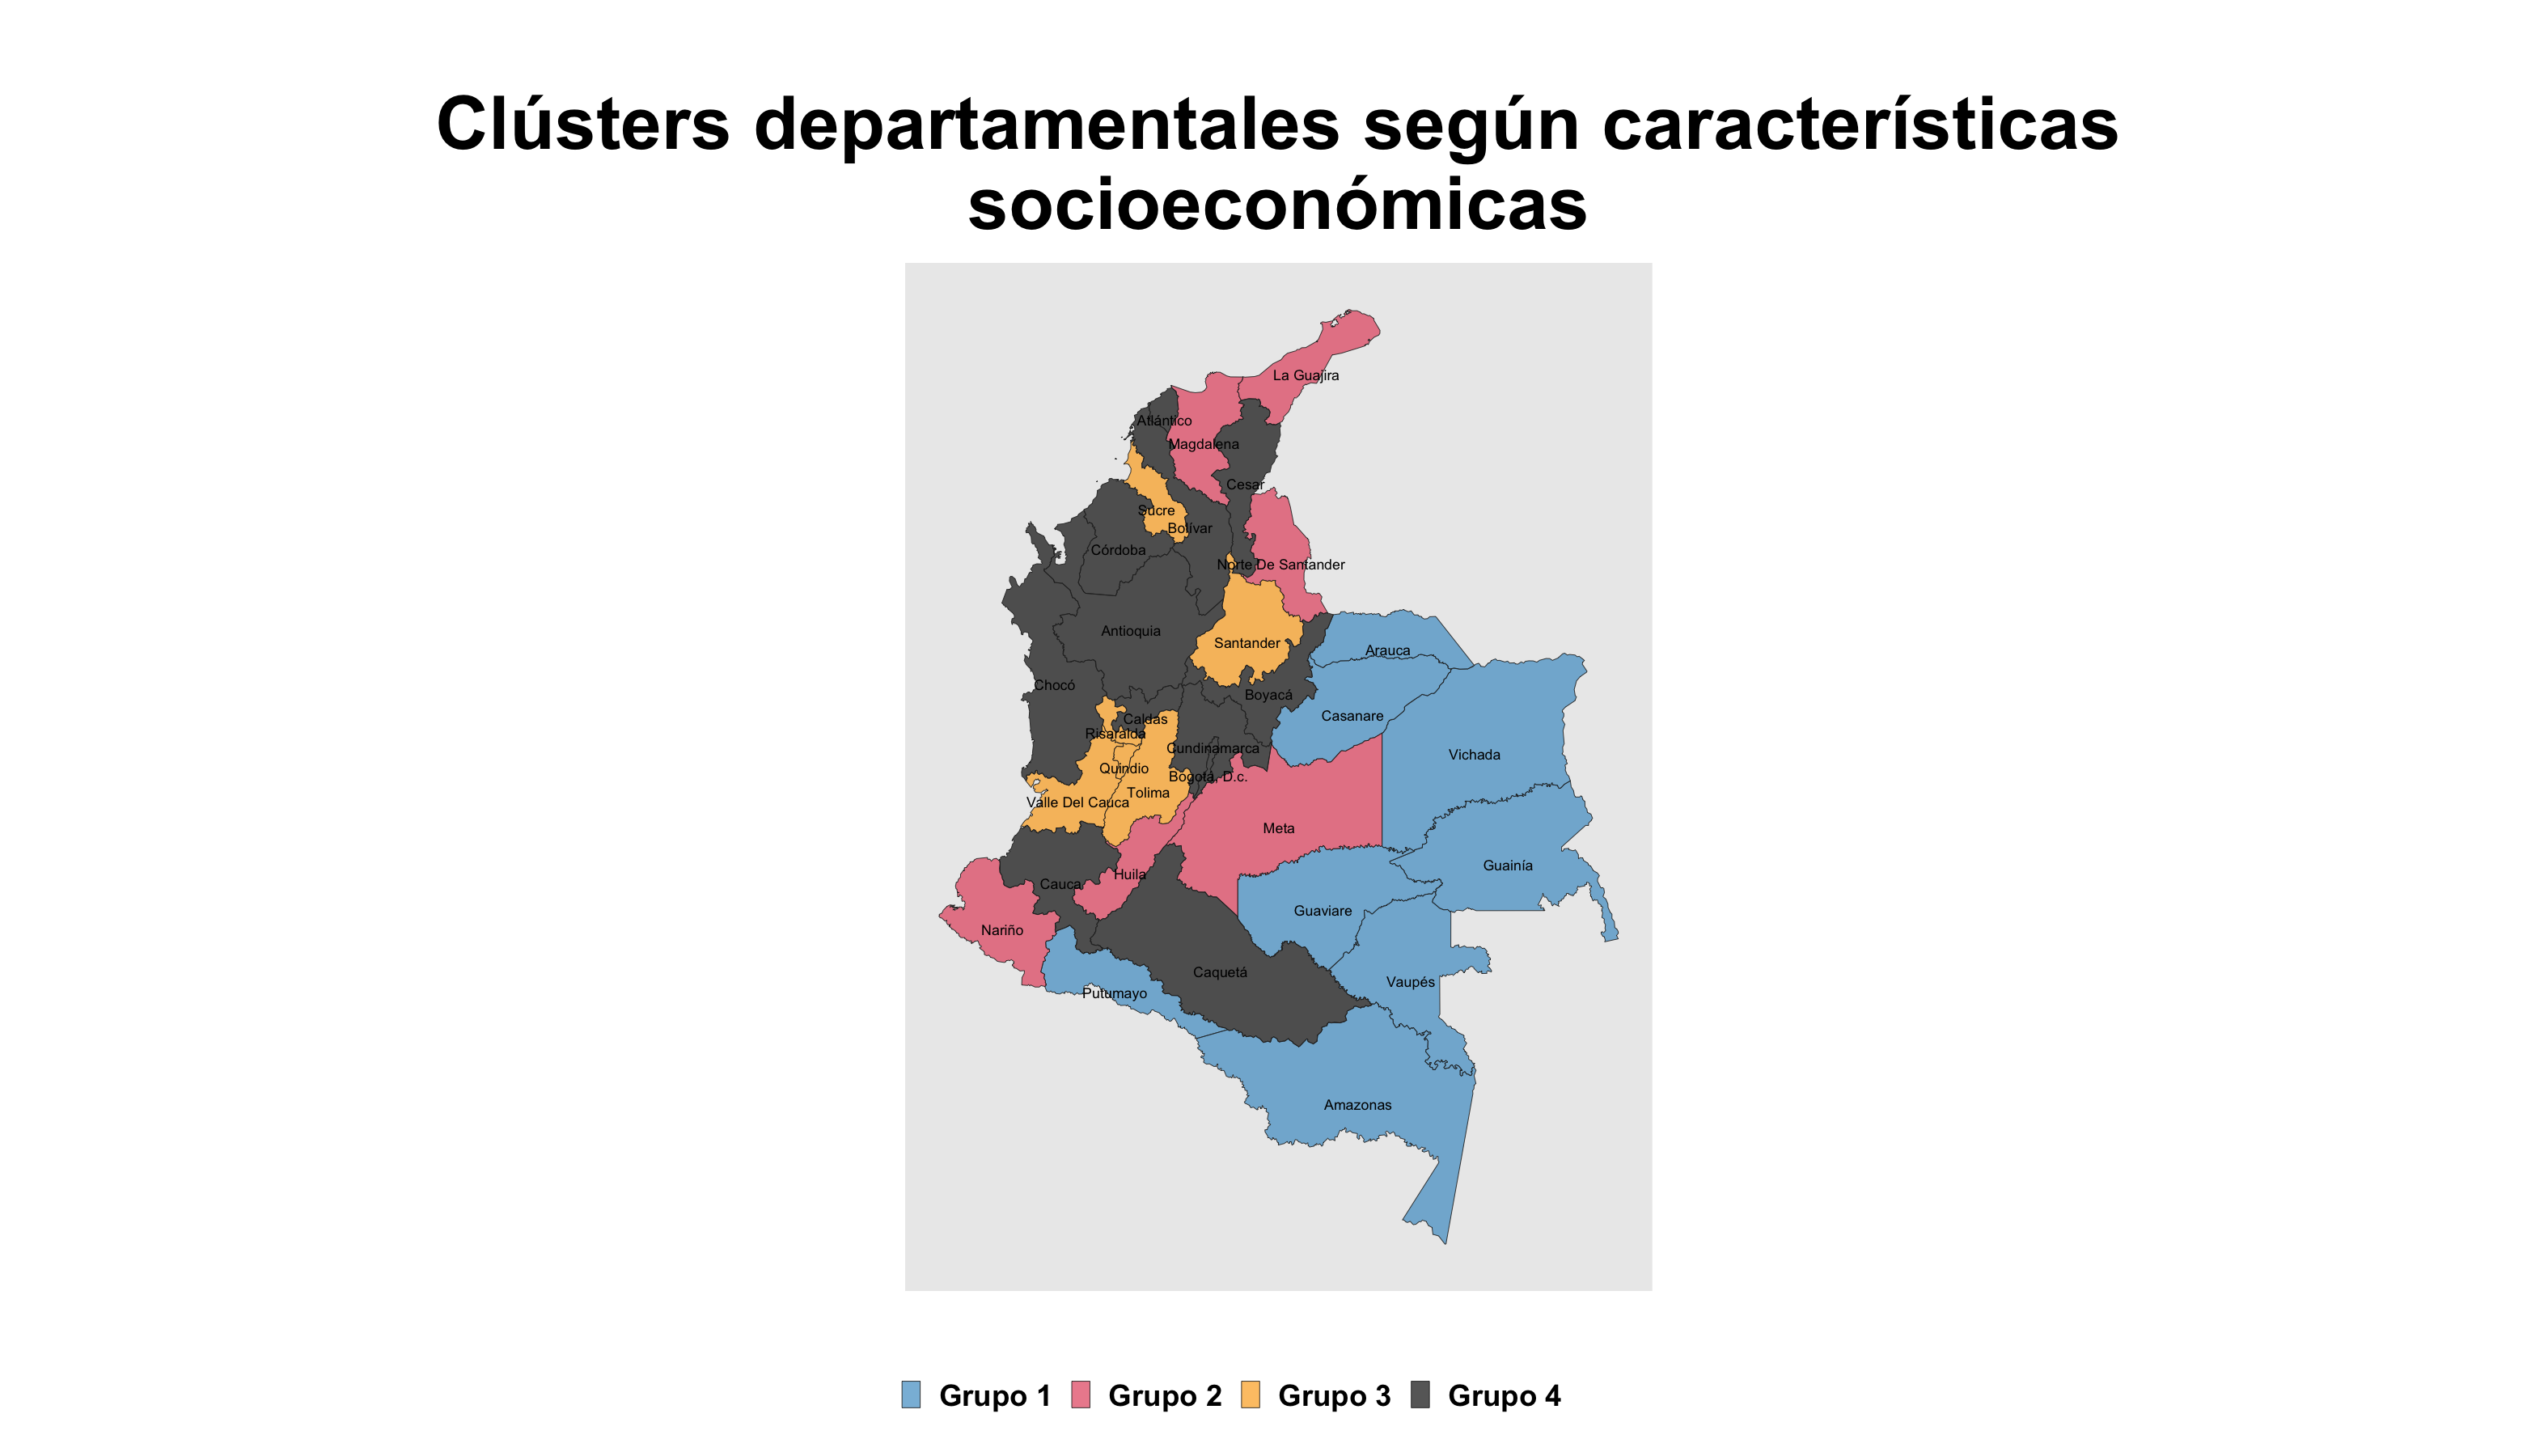
\includegraphics[width=\columnwidth]{img/cluster_main.png}
            \end{imagecolumn}
            \begin{textcolumn}
                \begin{itemize}
                    \item Índice por cada dimensión
                    \item 4 grupos de departamentos
                \end{itemize}
            \end{textcolumn}
    \printcolumns
    \end{slide}
    
        %%% Contexto
    \slidetitle{19}
    
    
   
\end{document}